\appendix

\chapter{Graphs for \secref{sec:empirical}}\label{sec:app}

This appendix contains graphs similar to the ones described in
\secref{sssect:graphs} for all 10 packages discussed in \secref{sec:empirical}.
There are 6 graphs per package: the top two show the relationship between the
method size and stability (left) or groundedness (right); the other four graphs
connect the two type-related properties with control-flow features: the number
of gotos and the number of returns in a method instance.

Note that the bottom four graphs for every package are different from the top
two in that they group method instances, not methods. Therefore,
the bottom four graphs have all data bins either at level $OY=0$ or $1$, because
we always know whether a method instance is stable (grounded) or not.
The change comes from the fact that the control-flow features in question
depend on compiled code and the way it was optimized: e.\;g., an \c{if true} in a
method can be optimized away during compilation.

\clearpage

\subsection{Package: DifferentialEquations}
\begin{figure}[h]
     \begin{subfigure}[b]{0.49\textwidth}
       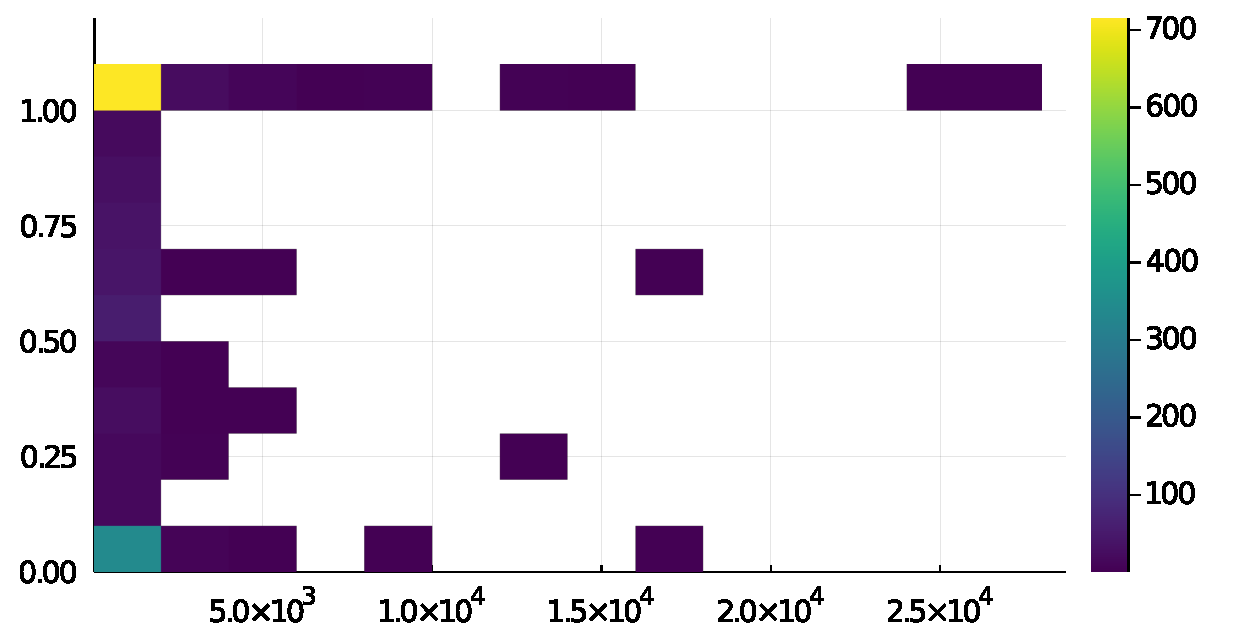
\includegraphics[width=\textwidth]{figs/all-package-graphs/DifferentialEquations-size-vs-stable.pdf}
     \end{subfigure}
     \ \
     \begin{subfigure}[b]{0.49\textwidth}
       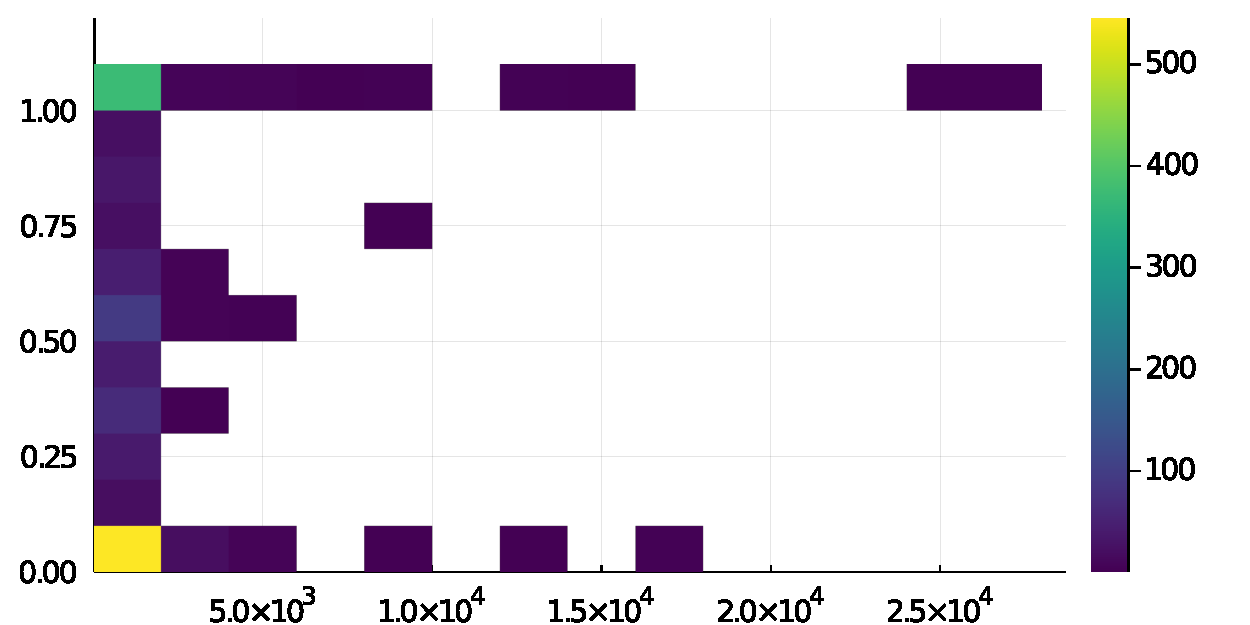
\includegraphics[width=\textwidth]{figs/all-package-graphs/DifferentialEquations-size-vs-grounded.pdf}
     \end{subfigure}
\caption{Stability (left, OY axis) and groundedness (right, OY) by method size (OX)}%
\Description{Stability and groundedness by method size in DifferentialEquations}%
\label{figs:size:DifferentialEquations}
\end{figure}

\begin{figure}[h]
     \begin{subfigure}[b]{0.49\textwidth}
       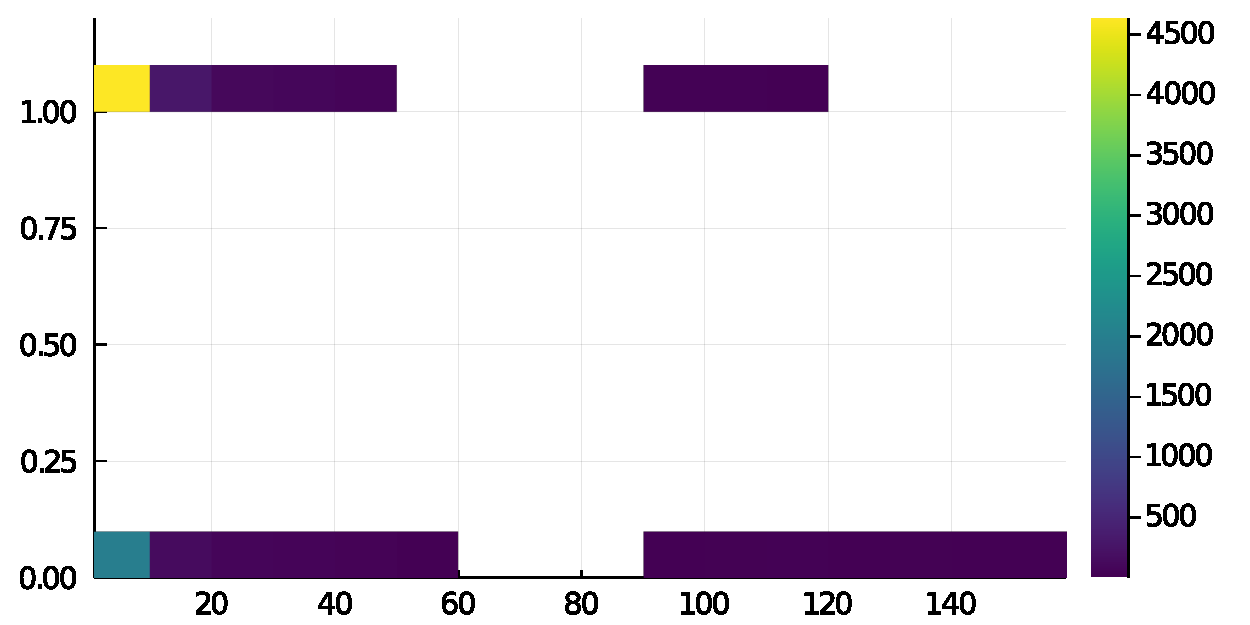
\includegraphics[width=\textwidth]{figs/all-package-graphs/DifferentialEquations-gotos-vs-stable.pdf}
     \end{subfigure}
     \ \
     \begin{subfigure}[b]{0.49\textwidth}
       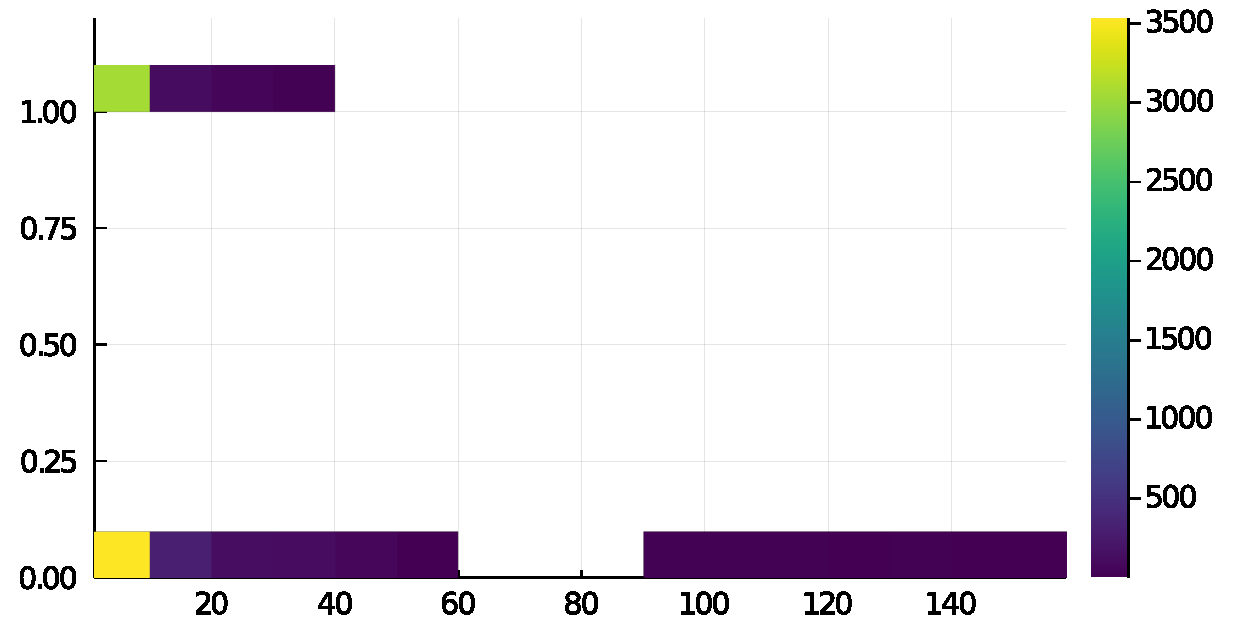
\includegraphics[width=\textwidth]{figs/all-package-graphs/DifferentialEquations-gotos-vs-grounded.pdf}
     \end{subfigure}
\caption{Stability (left, OY axis) and groundedness (right, OY) by number of gotos in method instances (OX)}%
\Description{Stability and groundedness by number of goto's in method instances in DifferentialEquations}%
\label{figs:gotos:DifferentialEquations}
\end{figure}

\begin{figure}[h]
     \begin{subfigure}[b]{0.49\textwidth}
       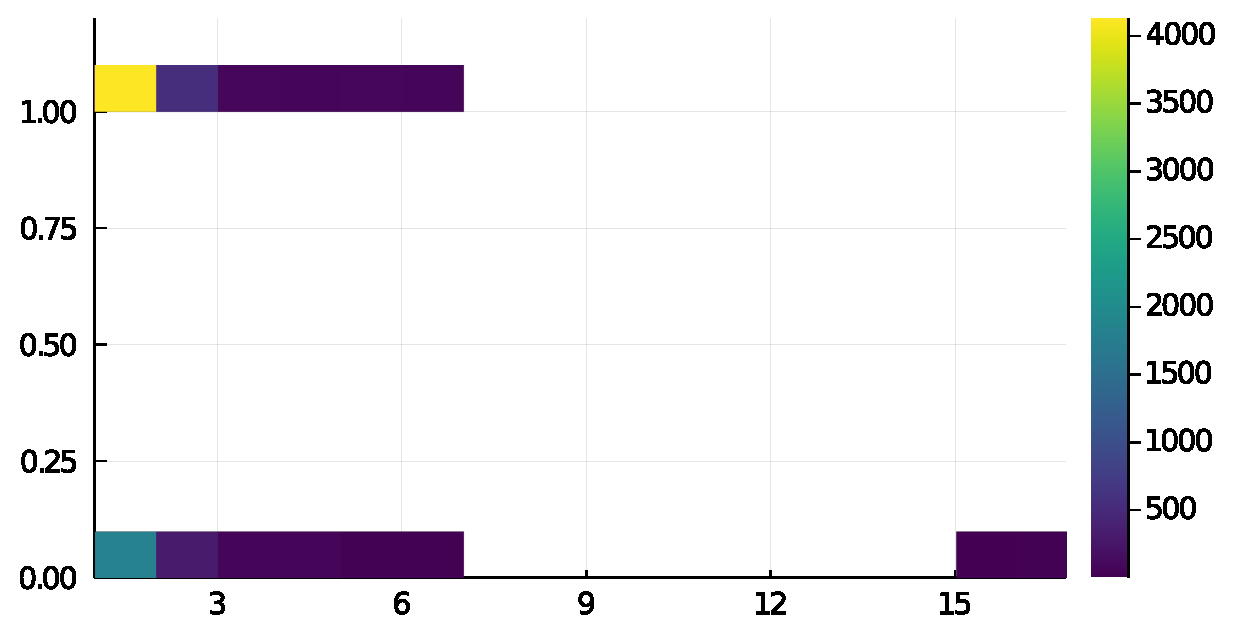
\includegraphics[width=\textwidth]{figs/all-package-graphs/DifferentialEquations-returns-vs-stable.pdf}
     \end{subfigure}
     \ \
     \begin{subfigure}[b]{0.49\textwidth}
       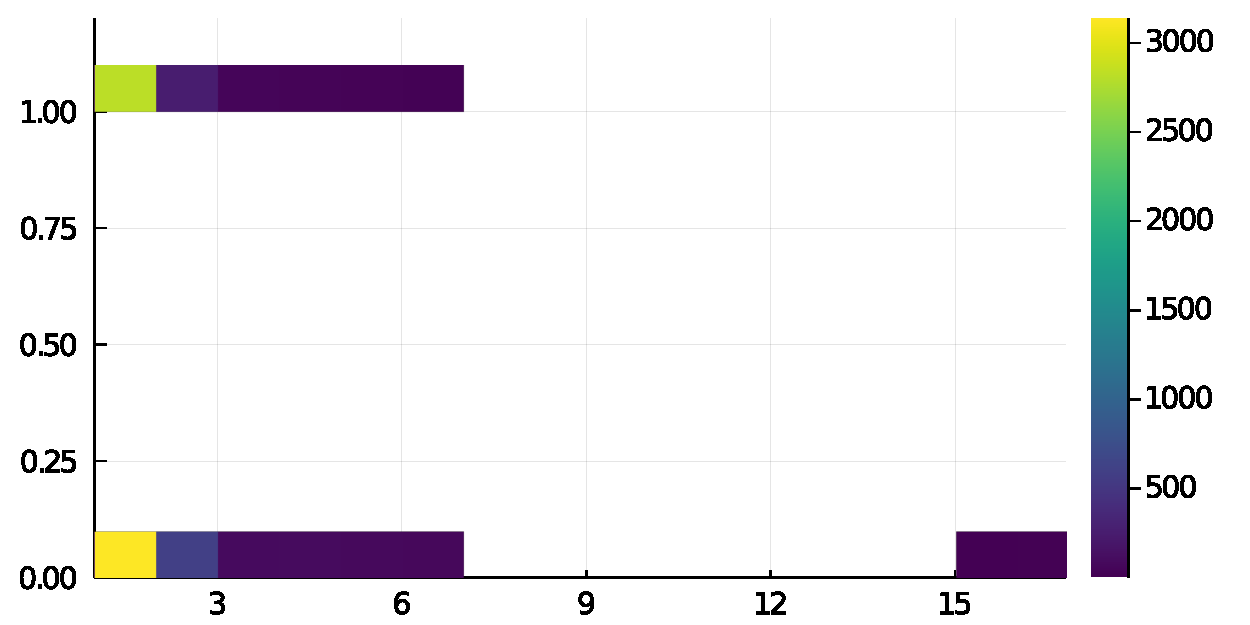
\includegraphics[width=\textwidth]{figs/all-package-graphs/DifferentialEquations-returns-vs-grounded.pdf}
     \end{subfigure}
\caption{Stability (left, OY axis) and groundedness (right, OY) by number of returns in method instances (OX)}%
\Description{Stability and groundedness by number of returns in method instances in DifferentialEquations}%
\label{figs:returns:DifferentialEquations}
\end{figure}
\clearpage
\subsection{Package: Flux}
\begin{figure}[h]
     \begin{subfigure}[b]{0.49\textwidth}
       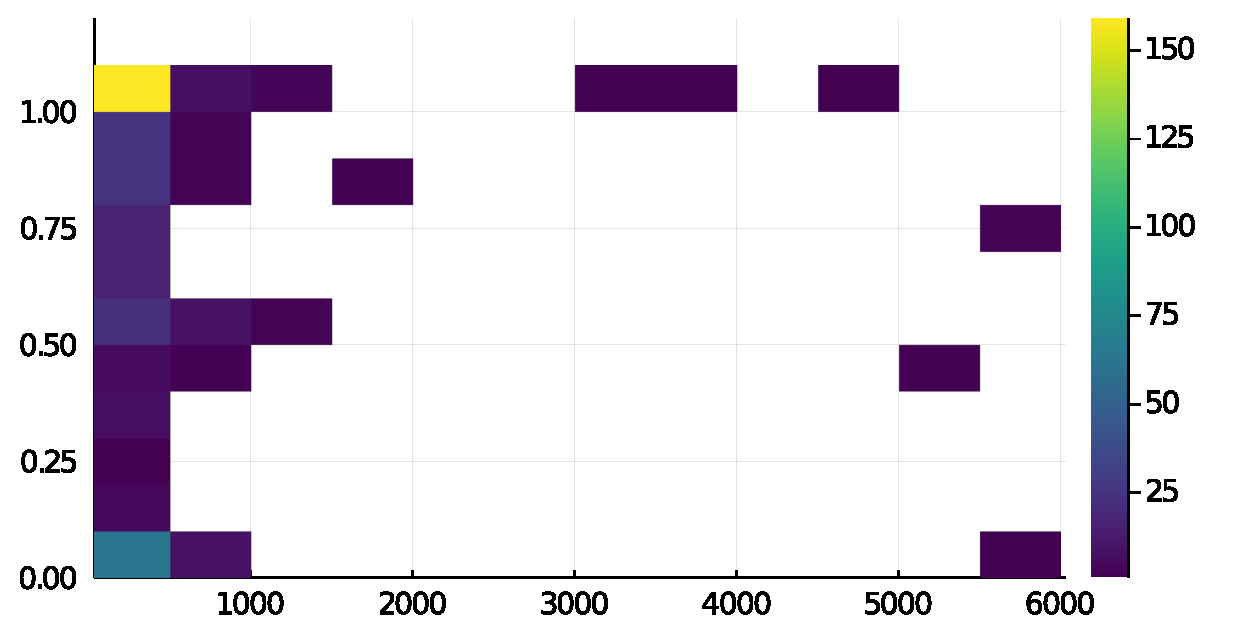
\includegraphics[width=\textwidth]{figs/all-package-graphs/Flux-size-vs-stable.pdf}
     \end{subfigure}
     \ \
     \begin{subfigure}[b]{0.49\textwidth}
       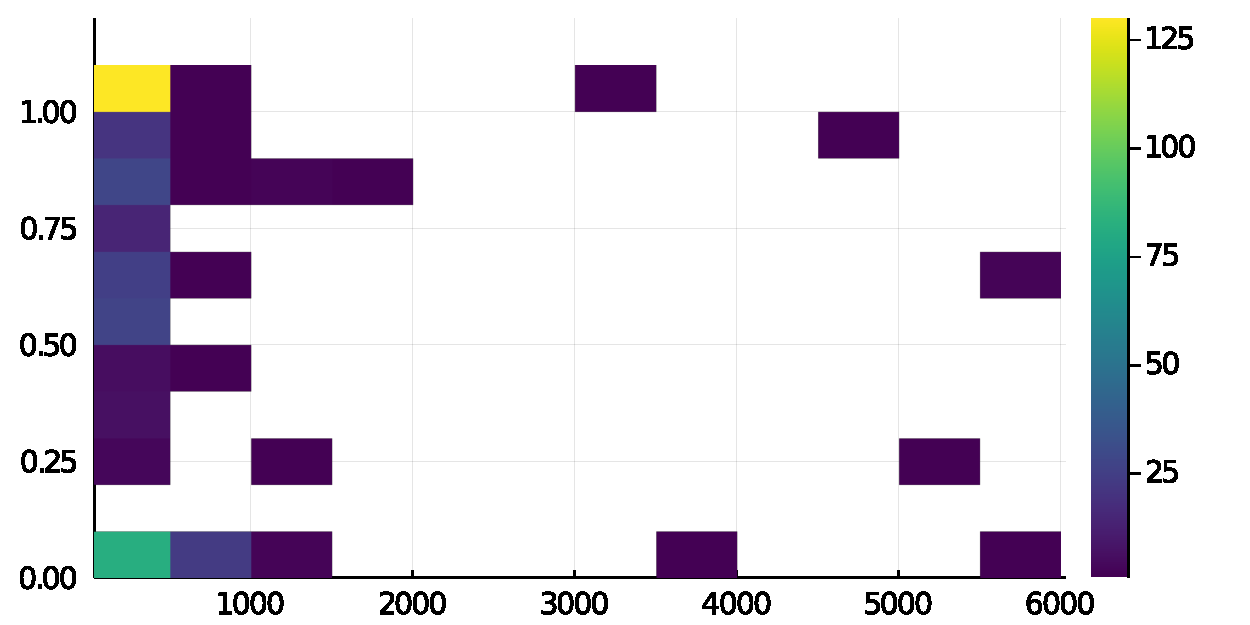
\includegraphics[width=\textwidth]{figs/all-package-graphs/Flux-size-vs-grounded.pdf}
     \end{subfigure}
\caption{Stability (left, OY axis) and groundedness (right, OY) by method size (OX)}%
\Description{Stability and groundedness by method size in Flux}%
\label{figs:size:Flux}
\end{figure}

\begin{figure}[h]
     \begin{subfigure}[b]{0.49\textwidth}
       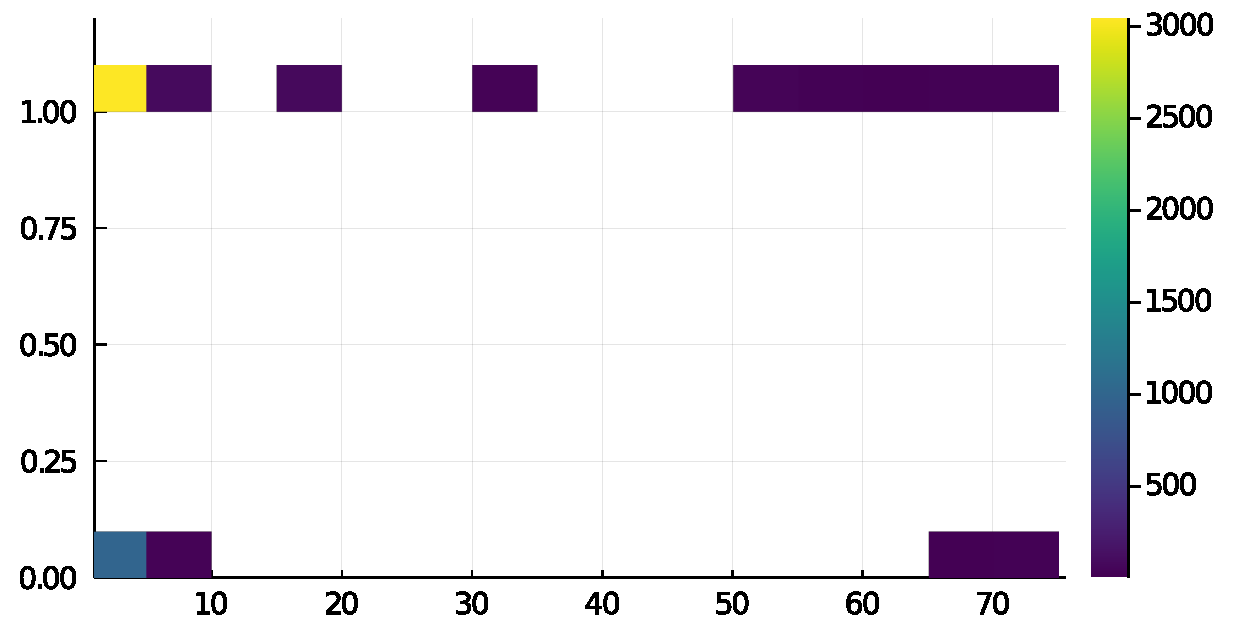
\includegraphics[width=\textwidth]{figs/all-package-graphs/Flux-gotos-vs-stable.pdf}
     \end{subfigure}
     \ \
     \begin{subfigure}[b]{0.49\textwidth}
       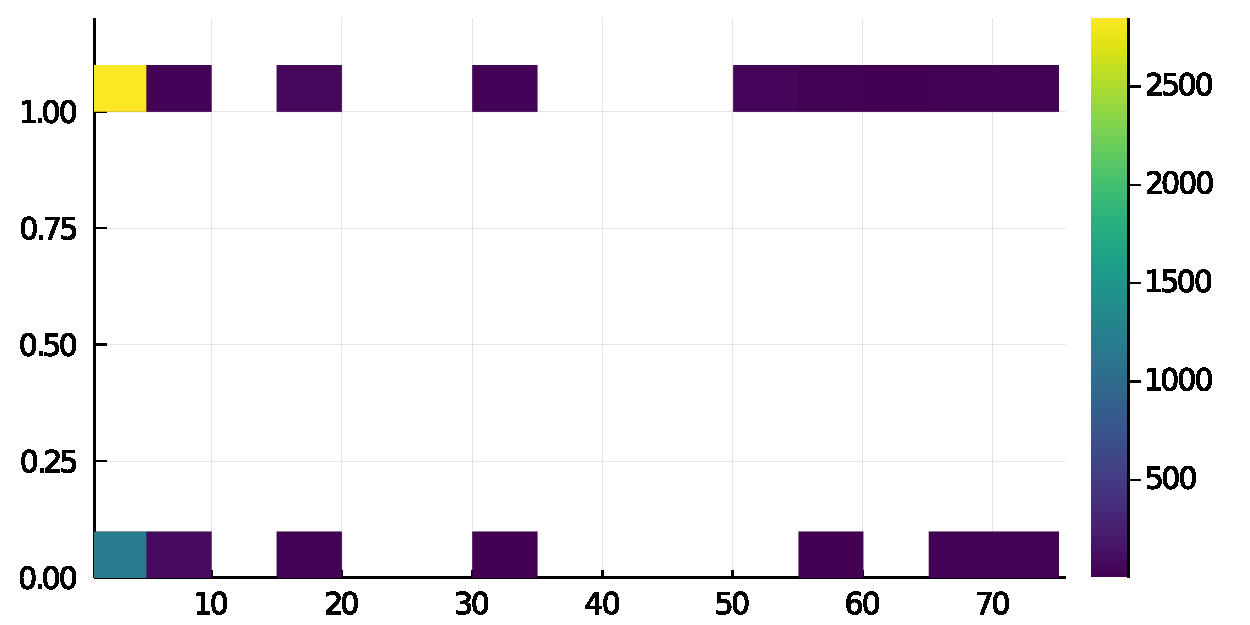
\includegraphics[width=\textwidth]{figs/all-package-graphs/Flux-gotos-vs-grounded.pdf}
     \end{subfigure}
\caption{Stability (left, OY axis) and groundedness (right, OY) by number of gotos in method instances (OX)}%
\Description{Stability and groundedness by number of goto's in method instances in Flux}%
\label{figs:gotos:Flux}
\end{figure}

\begin{figure}[h]
     \begin{subfigure}[b]{0.49\textwidth}
       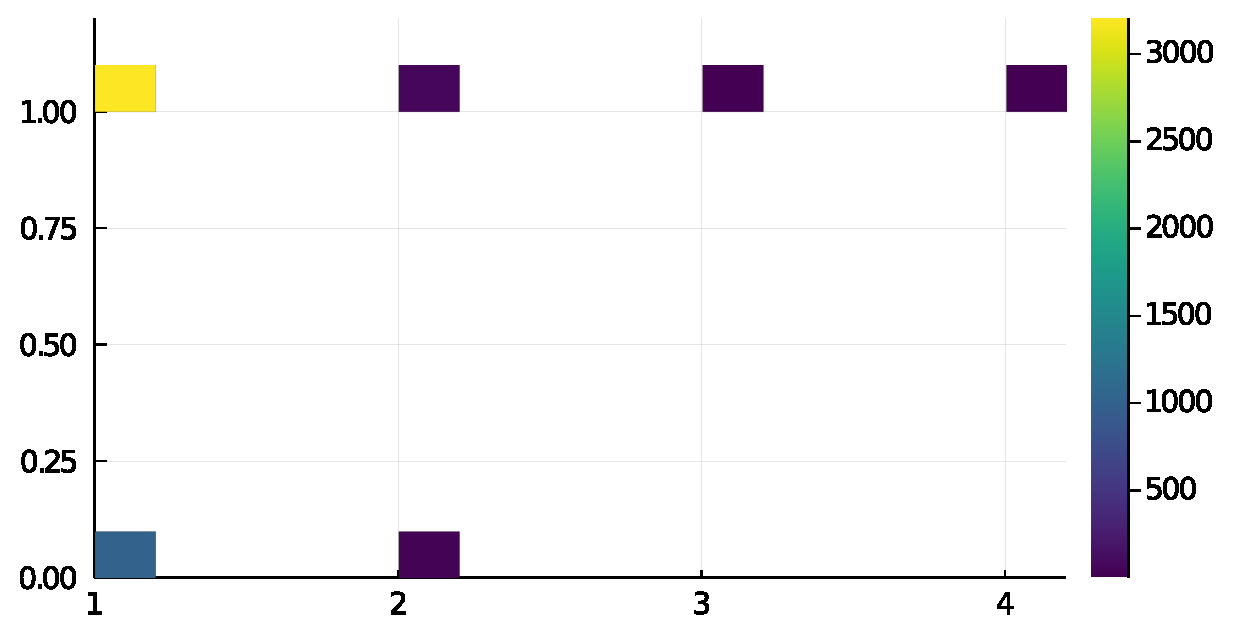
\includegraphics[width=\textwidth]{figs/all-package-graphs/Flux-returns-vs-stable.pdf}
     \end{subfigure}
     \ \
     \begin{subfigure}[b]{0.49\textwidth}
       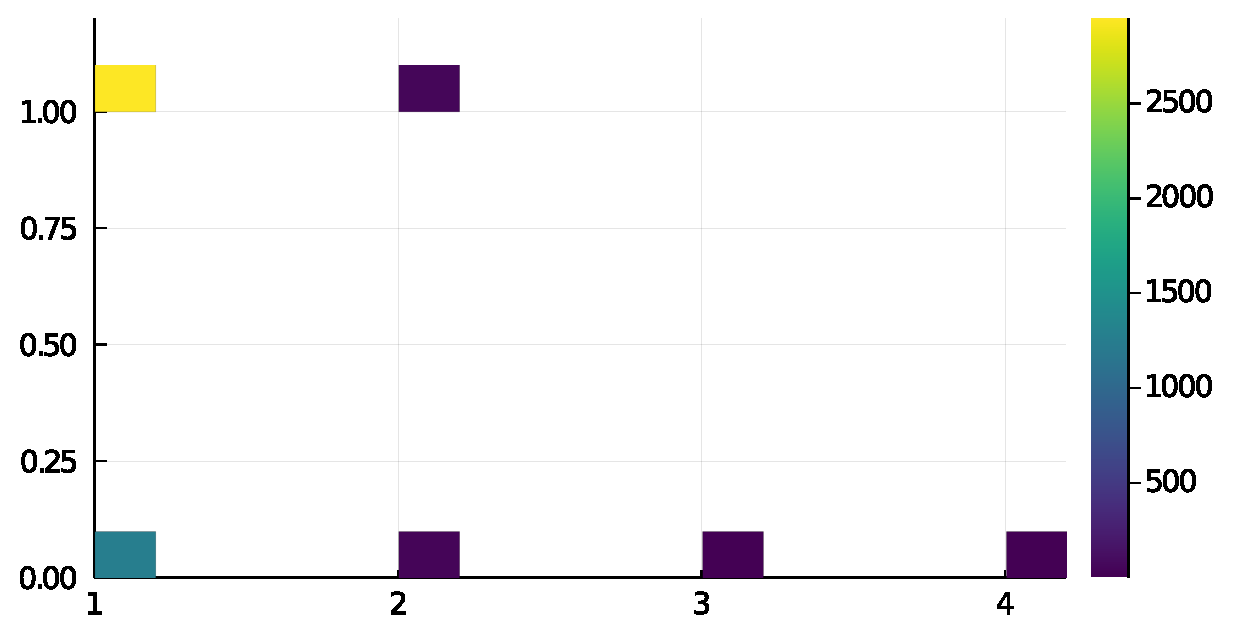
\includegraphics[width=\textwidth]{figs/all-package-graphs/Flux-returns-vs-grounded.pdf}
     \end{subfigure}
\caption{Stability (left, OY axis) and groundedness (right, OY) by number of returns in method instances (OX)}%
\Description{Stability and groundedness by number of returns in method instances in Flux}%
\label{figs:returns:Flux}
\end{figure}
\clearpage
\subsection{Package: Gadfly}
\begin{figure}[h]
     \begin{subfigure}[b]{0.49\textwidth}
       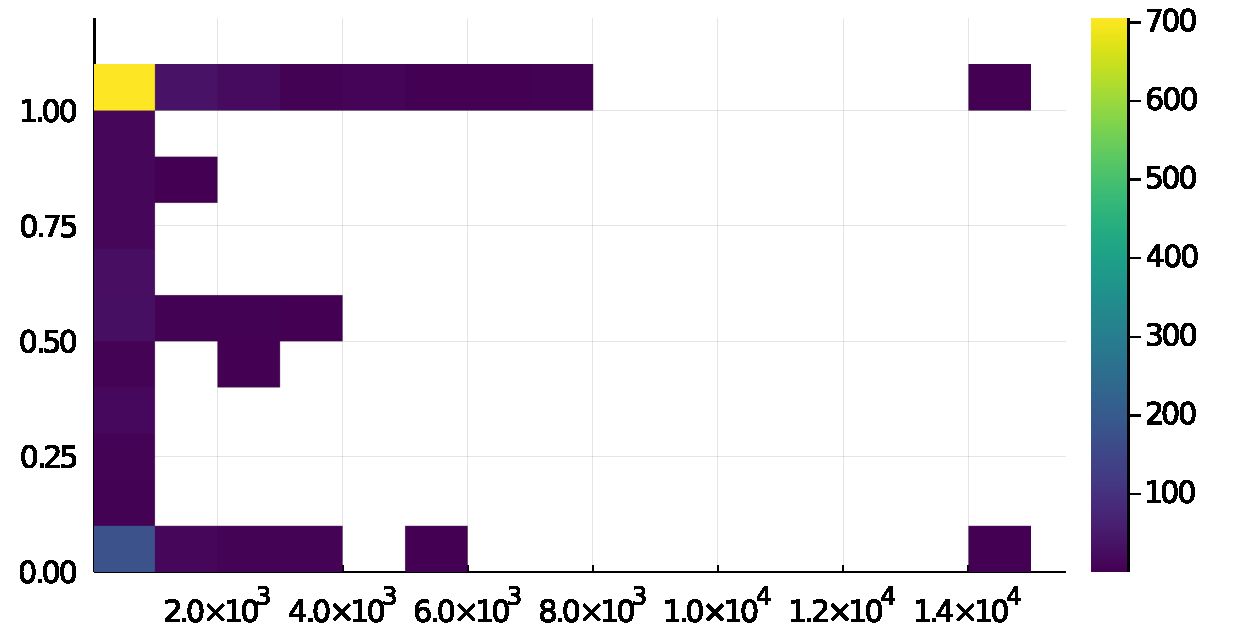
\includegraphics[width=\textwidth]{figs/all-package-graphs/Gadfly-size-vs-stable.pdf}
     \end{subfigure}
     \ \
     \begin{subfigure}[b]{0.49\textwidth}
       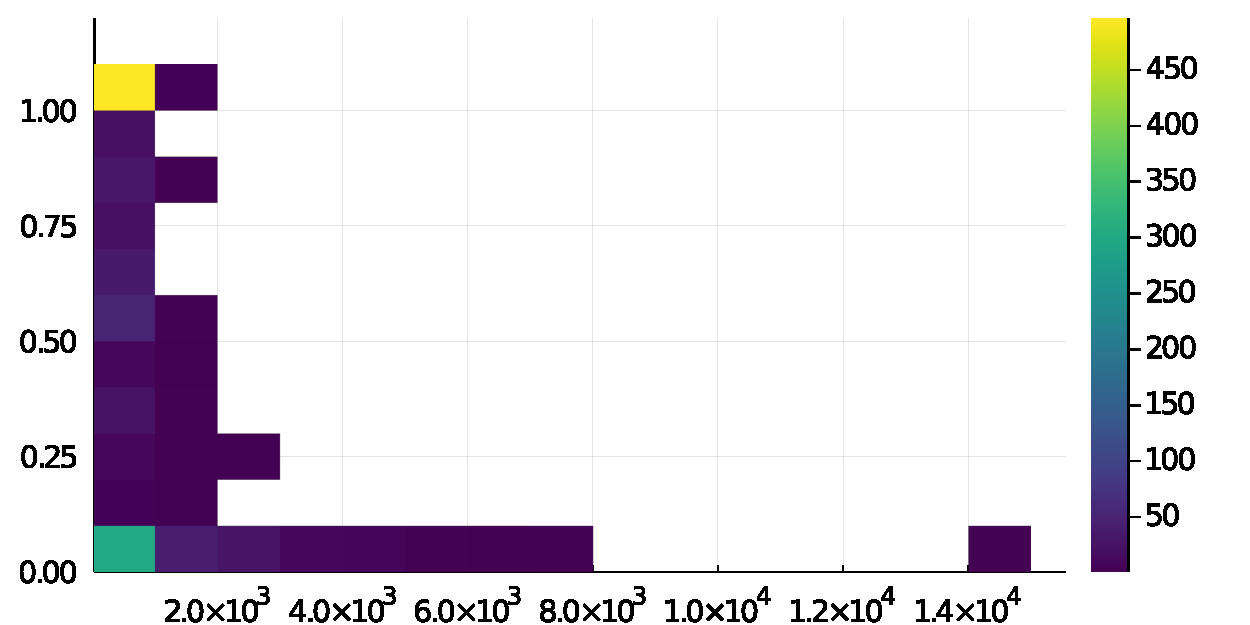
\includegraphics[width=\textwidth]{figs/all-package-graphs/Gadfly-size-vs-grounded.pdf}
     \end{subfigure}
\caption{Stability (left, OY axis) and groundedness (right, OY) by method size (OX)}%
\Description{Stability and groundedness by method size in Gadfly}%
\label{figs:size:Gadfly}
\end{figure}

\begin{figure}[h]
     \begin{subfigure}[b]{0.49\textwidth}
       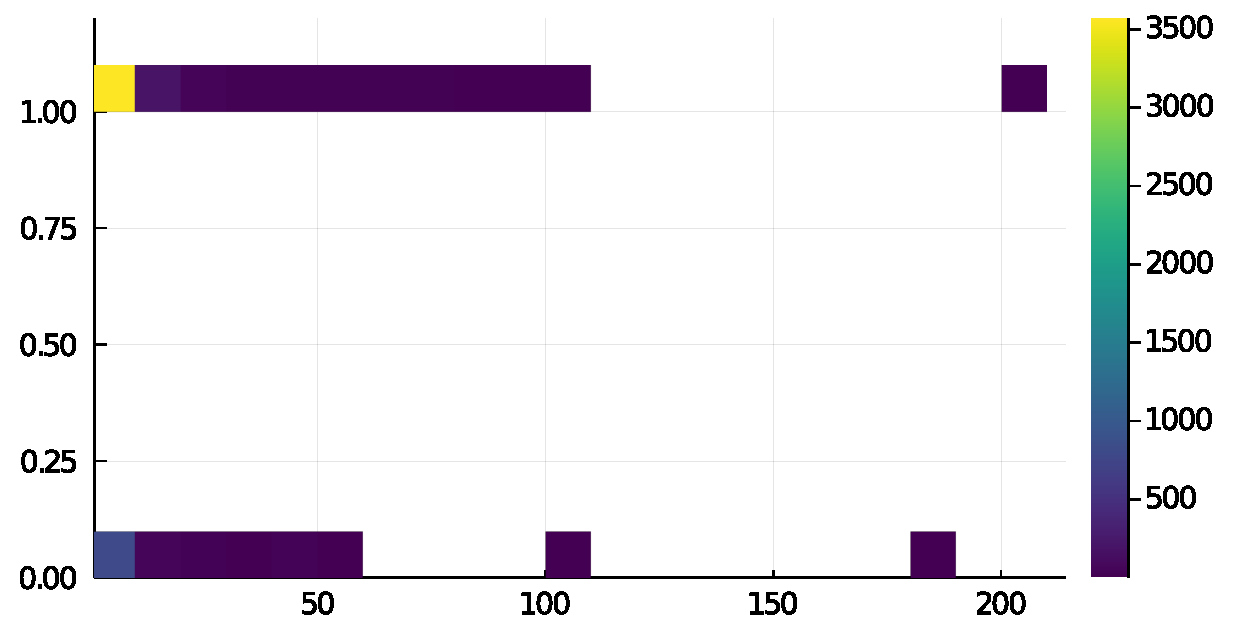
\includegraphics[width=\textwidth]{figs/all-package-graphs/Gadfly-gotos-vs-stable.pdf}
     \end{subfigure}
     \ \
     \begin{subfigure}[b]{0.49\textwidth}
       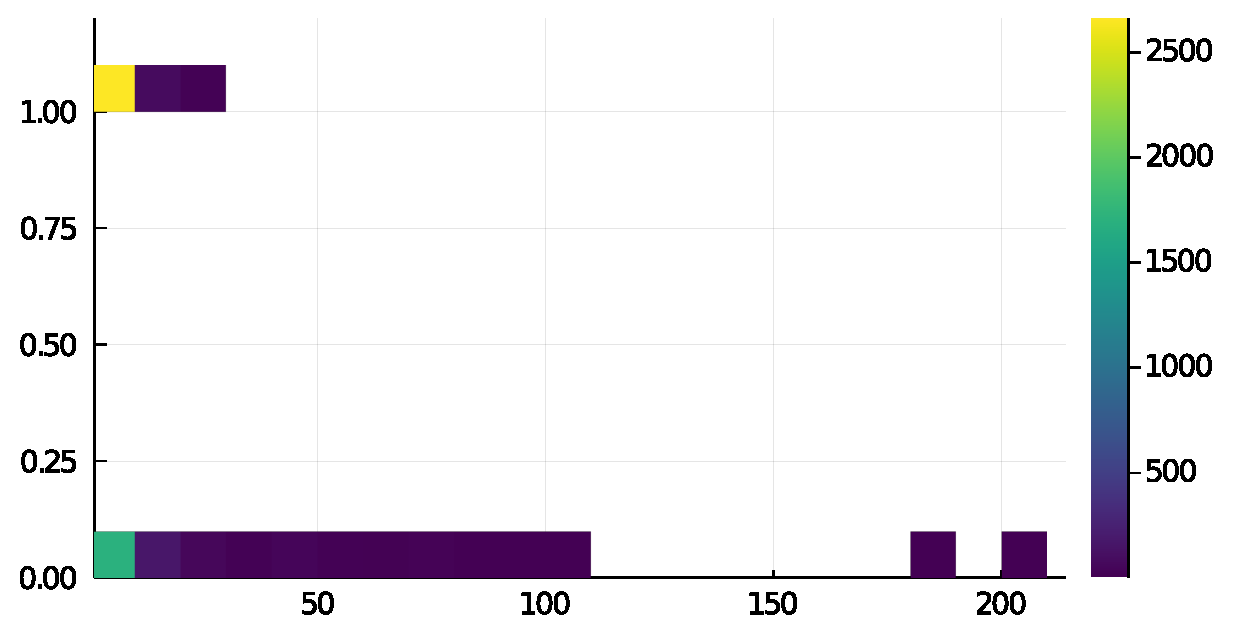
\includegraphics[width=\textwidth]{figs/all-package-graphs/Gadfly-gotos-vs-grounded.pdf}
     \end{subfigure}
\caption{Stability (left, OY axis) and groundedness (right, OY) by number of gotos in method instances (OX)}%
\Description{Stability and groundedness by number of goto's in method instances in Gadfly}%
\label{figs:gotos:Gadfly}
\end{figure}

\begin{figure}[h]
     \begin{subfigure}[b]{0.49\textwidth}
       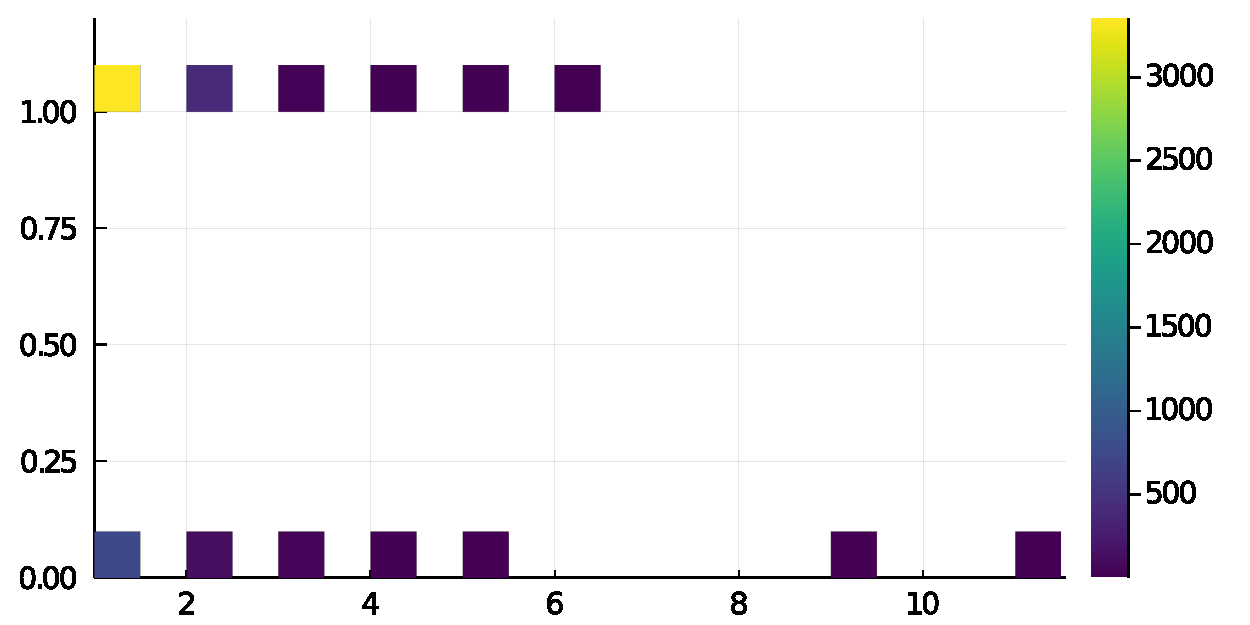
\includegraphics[width=\textwidth]{figs/all-package-graphs/Gadfly-returns-vs-stable.pdf}
     \end{subfigure}
     \ \
     \begin{subfigure}[b]{0.49\textwidth}
       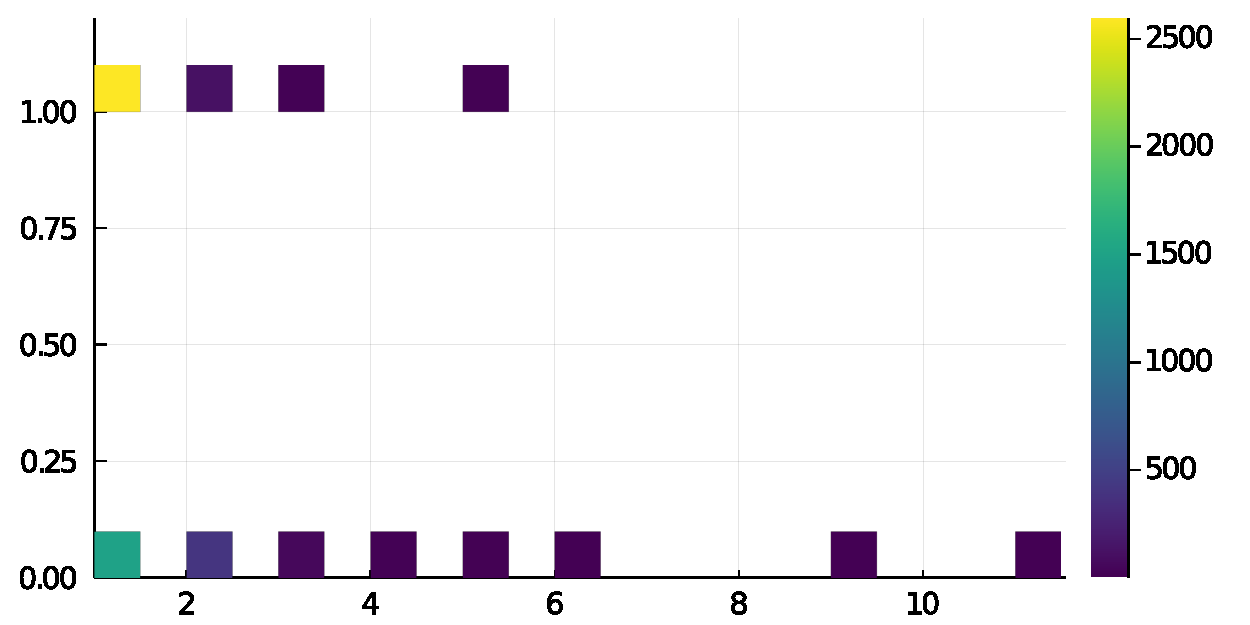
\includegraphics[width=\textwidth]{figs/all-package-graphs/Gadfly-returns-vs-grounded.pdf}
     \end{subfigure}
\caption{Stability (left, OY axis) and groundedness (right, OY) by number of returns in method instances (OX)}%
\Description{Stability and groundedness by number of returns in method instances in Gadfly}%
\label{figs:returns:Gadfly}
\end{figure}
\clearpage
\subsection{Package: Gen}
\begin{figure}[h]
     \begin{subfigure}[b]{0.49\textwidth}
       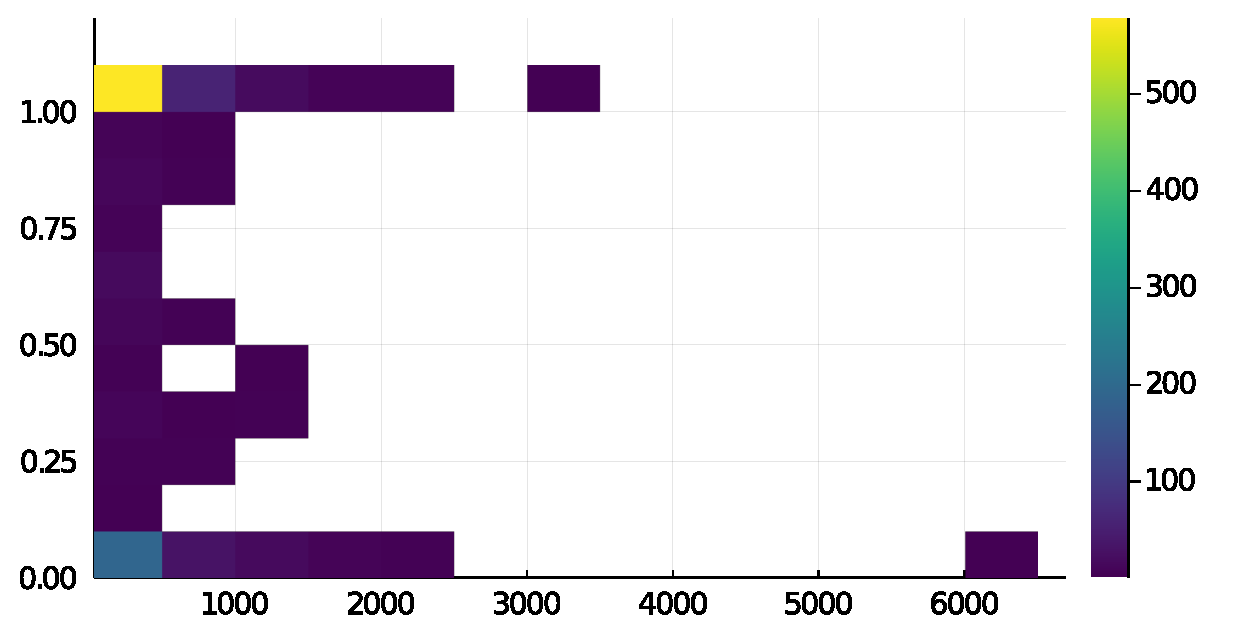
\includegraphics[width=\textwidth]{figs/all-package-graphs/Gen-size-vs-stable.pdf}
     \end{subfigure}
     \ \
     \begin{subfigure}[b]{0.49\textwidth}
       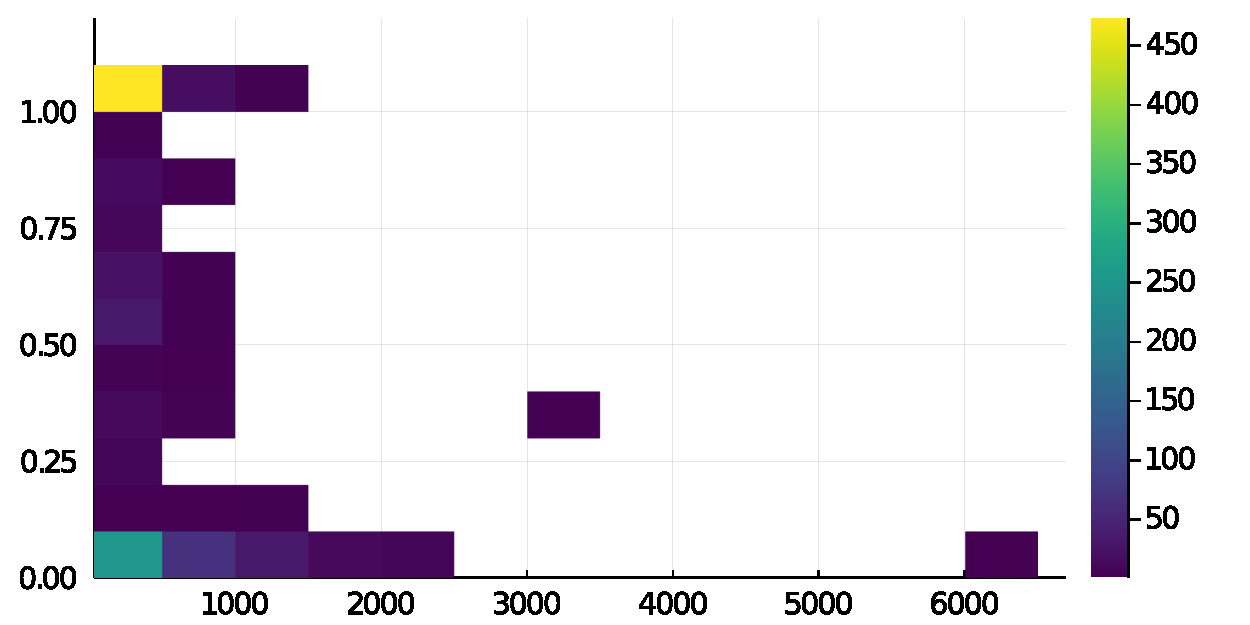
\includegraphics[width=\textwidth]{figs/all-package-graphs/Gen-size-vs-grounded.pdf}
     \end{subfigure}
\caption{Stability (left, OY axis) and groundedness (right, OY) by method size (OX)}%
\Description{Stability and groundedness by method size in Gen}%
\label{figs:size:Gen}
\end{figure}

\begin{figure}[h]
     \begin{subfigure}[b]{0.49\textwidth}
       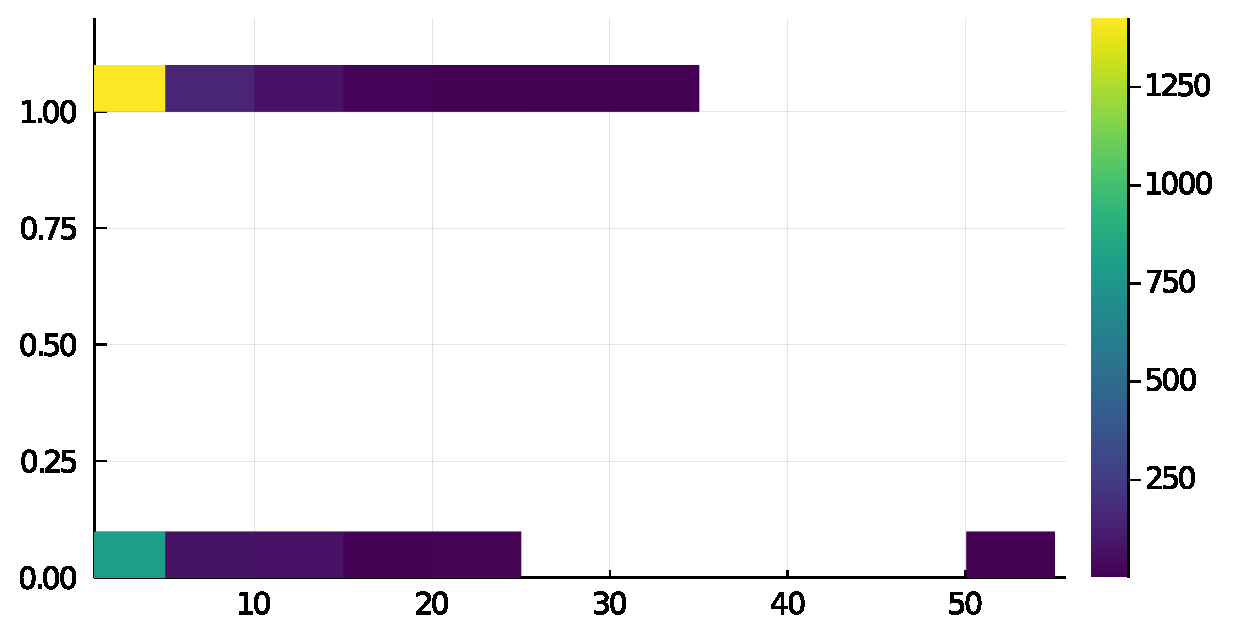
\includegraphics[width=\textwidth]{figs/all-package-graphs/Gen-gotos-vs-stable.pdf}
     \end{subfigure}
     \ \
     \begin{subfigure}[b]{0.49\textwidth}
       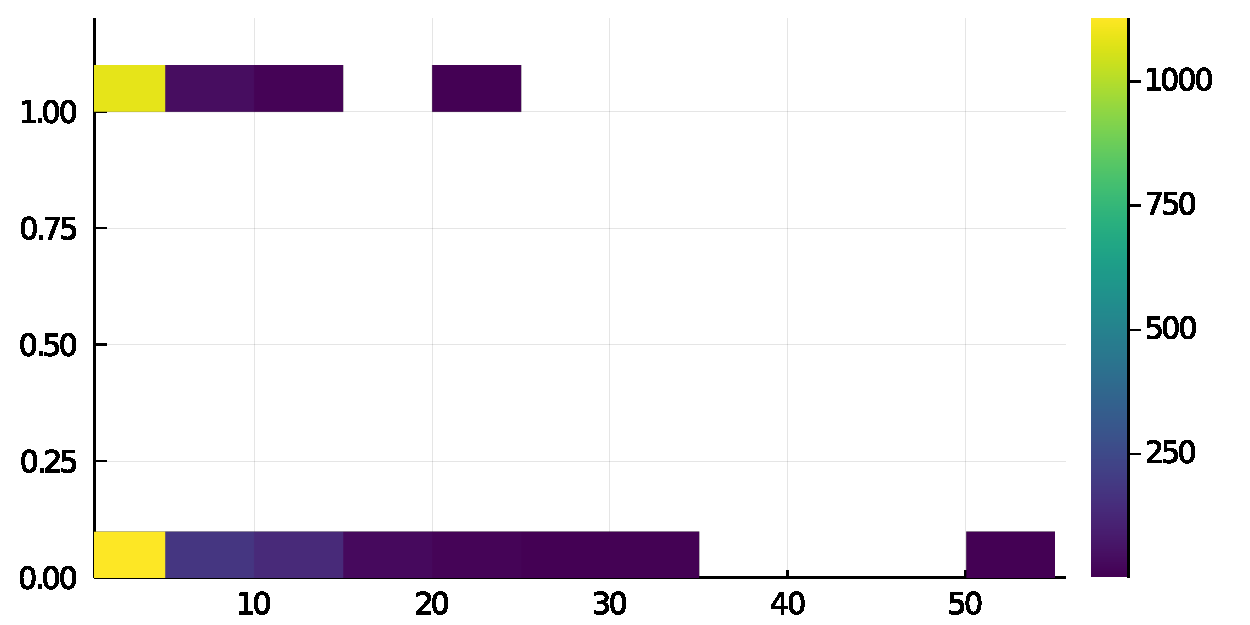
\includegraphics[width=\textwidth]{figs/all-package-graphs/Gen-gotos-vs-grounded.pdf}
     \end{subfigure}
\caption{Stability (left, OY axis) and groundedness (right, OY) by number of gotos in method instances (OX)}%
\Description{Stability and groundedness by number of goto's in method instances in Gen}%
\label{figs:gotos:Gen}
\end{figure}

\begin{figure}[h]
     \begin{subfigure}[b]{0.49\textwidth}
       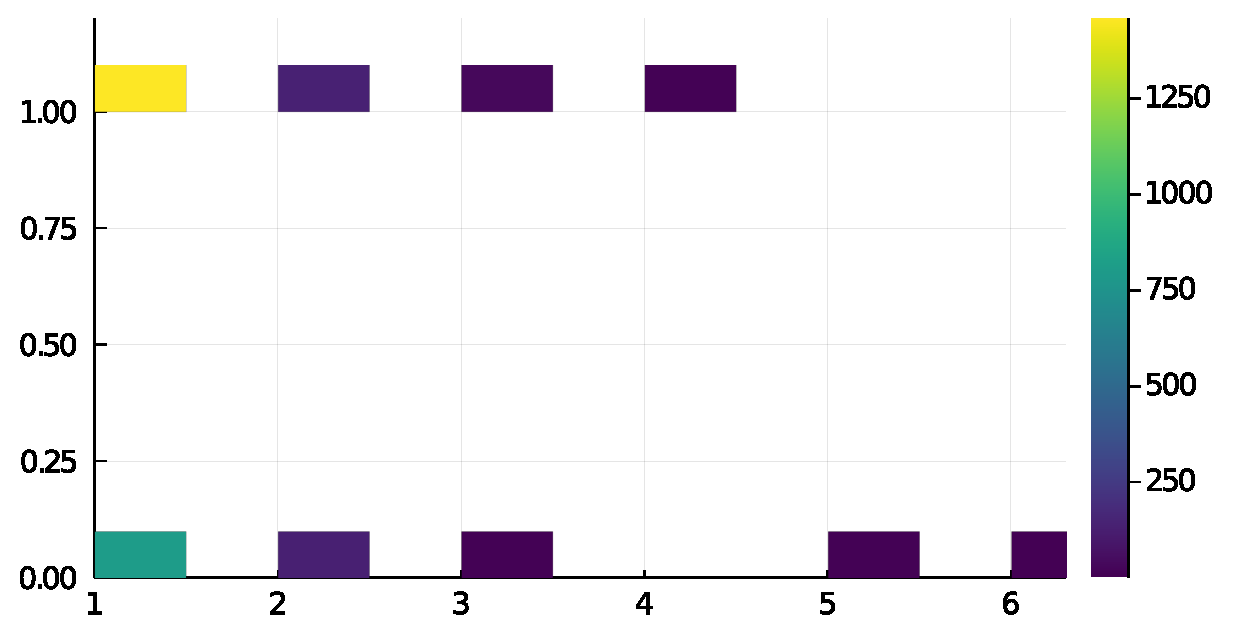
\includegraphics[width=\textwidth]{figs/all-package-graphs/Gen-returns-vs-stable.pdf}
     \end{subfigure}
     \ \
     \begin{subfigure}[b]{0.49\textwidth}
       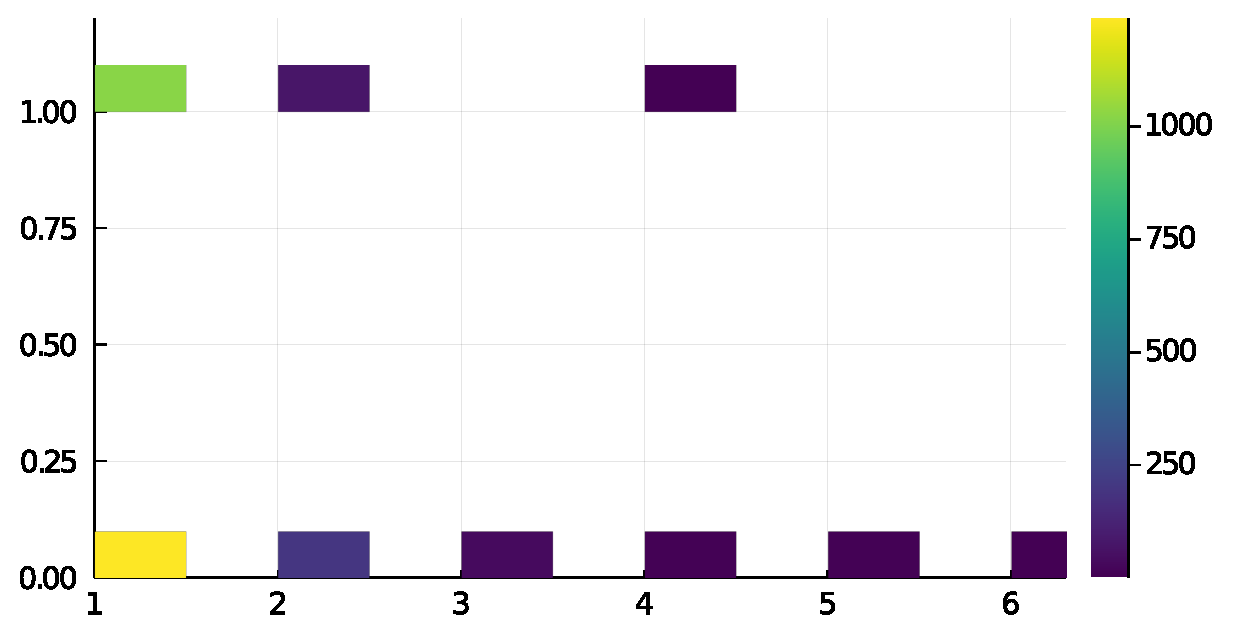
\includegraphics[width=\textwidth]{figs/all-package-graphs/Gen-returns-vs-grounded.pdf}
     \end{subfigure}
\caption{Stability (left, OY axis) and groundedness (right, OY) by number of returns in method instances (OX)}%
\Description{Stability and groundedness by number of returns in method instances in Gen}%
\label{figs:returns:Gen}
\end{figure}
\clearpage
\subsection{Package: Genie}
\begin{figure}[h]
     \begin{subfigure}[b]{0.49\textwidth}
       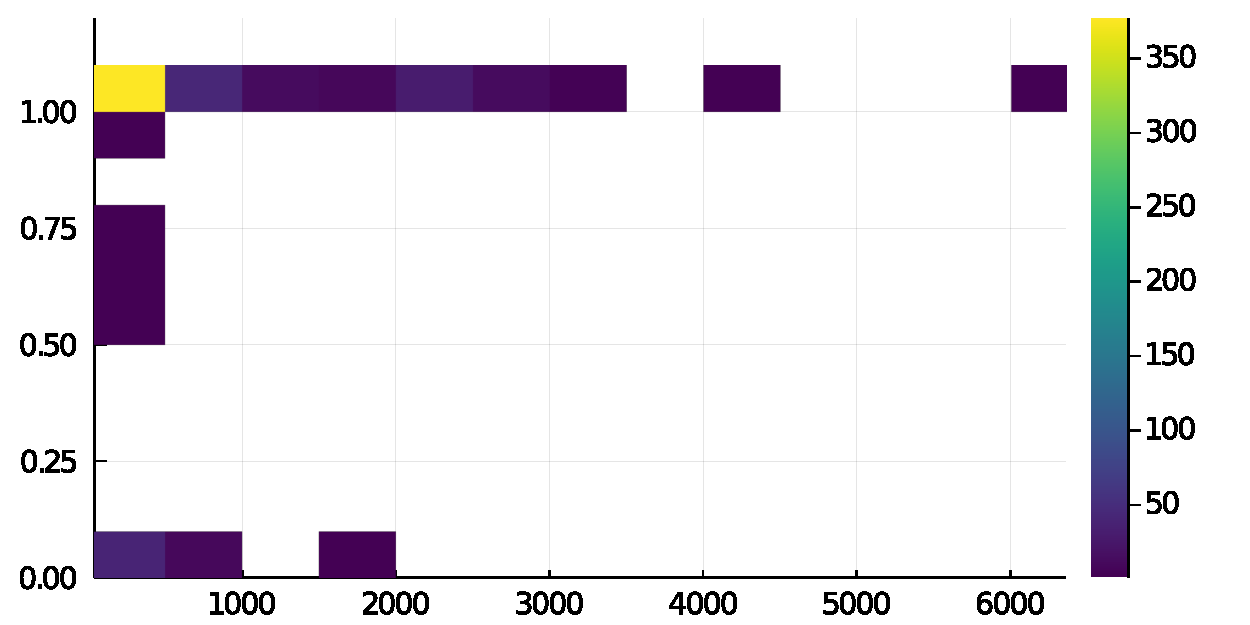
\includegraphics[width=\textwidth]{figs/all-package-graphs/Genie-size-vs-stable.pdf}
     \end{subfigure}
     \ \
     \begin{subfigure}[b]{0.49\textwidth}
       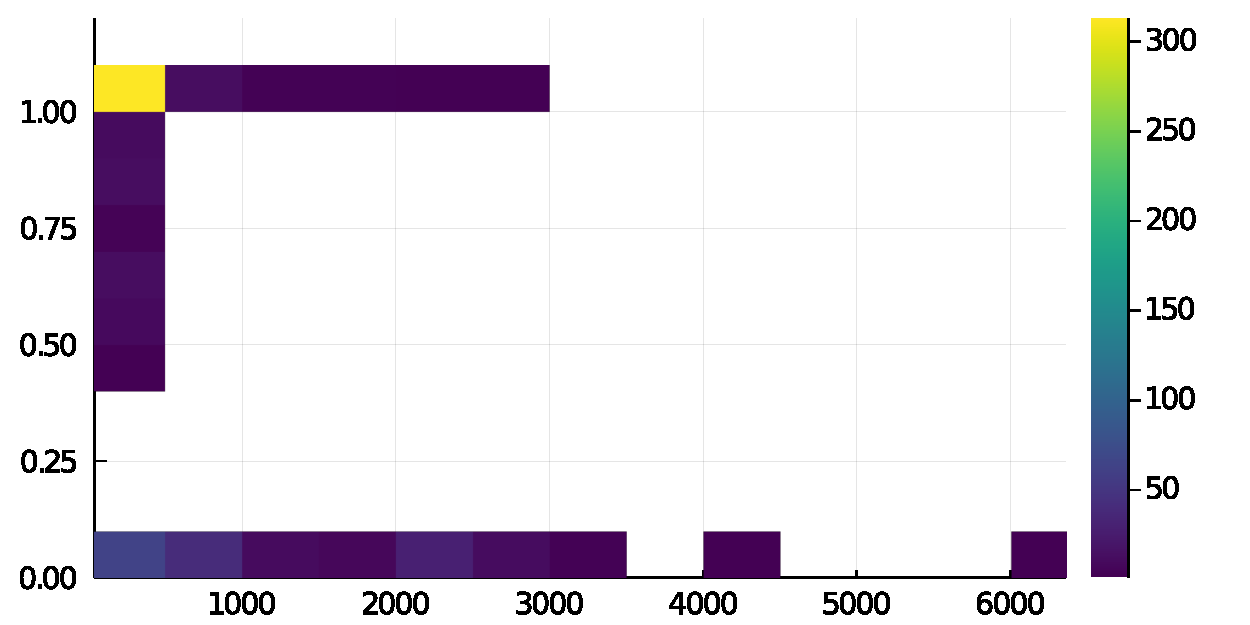
\includegraphics[width=\textwidth]{figs/all-package-graphs/Genie-size-vs-grounded.pdf}
     \end{subfigure}
\caption{Stability (left, OY axis) and groundedness (right, OY) by method size (OX)}%
\Description{Stability and groundedness by method size in Genie}%
\label{figs:size:Genie}
\end{figure}

\begin{figure}[h]
     \begin{subfigure}[b]{0.49\textwidth}
       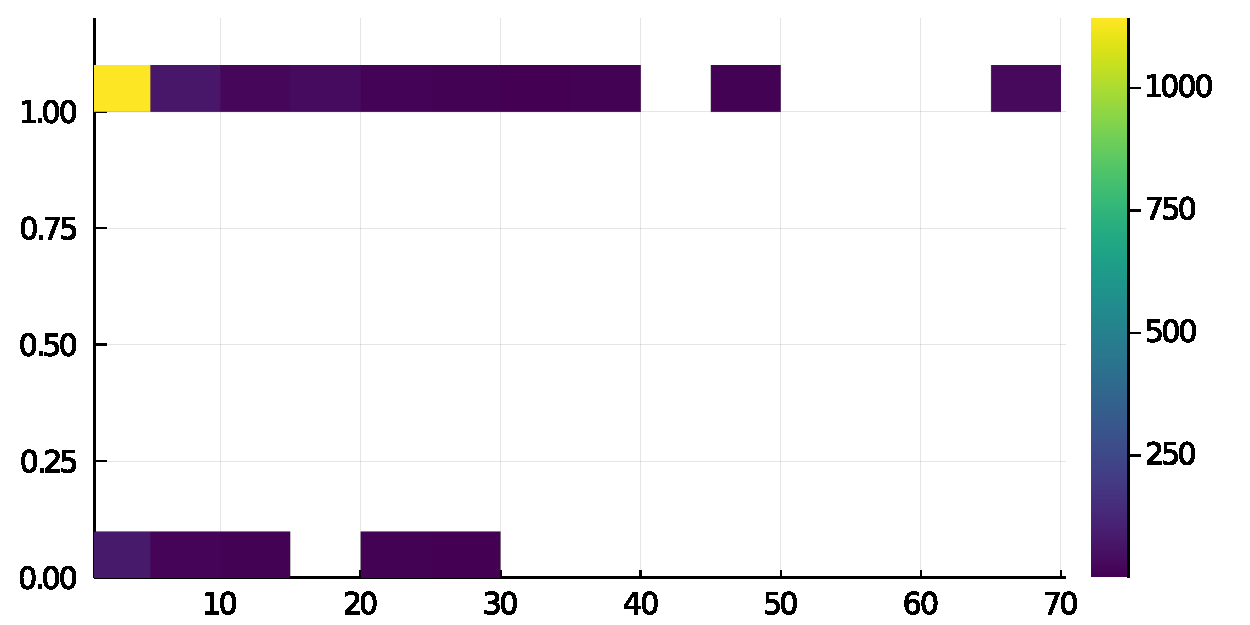
\includegraphics[width=\textwidth]{figs/all-package-graphs/Genie-gotos-vs-stable.pdf}
     \end{subfigure}
     \ \
     \begin{subfigure}[b]{0.49\textwidth}
       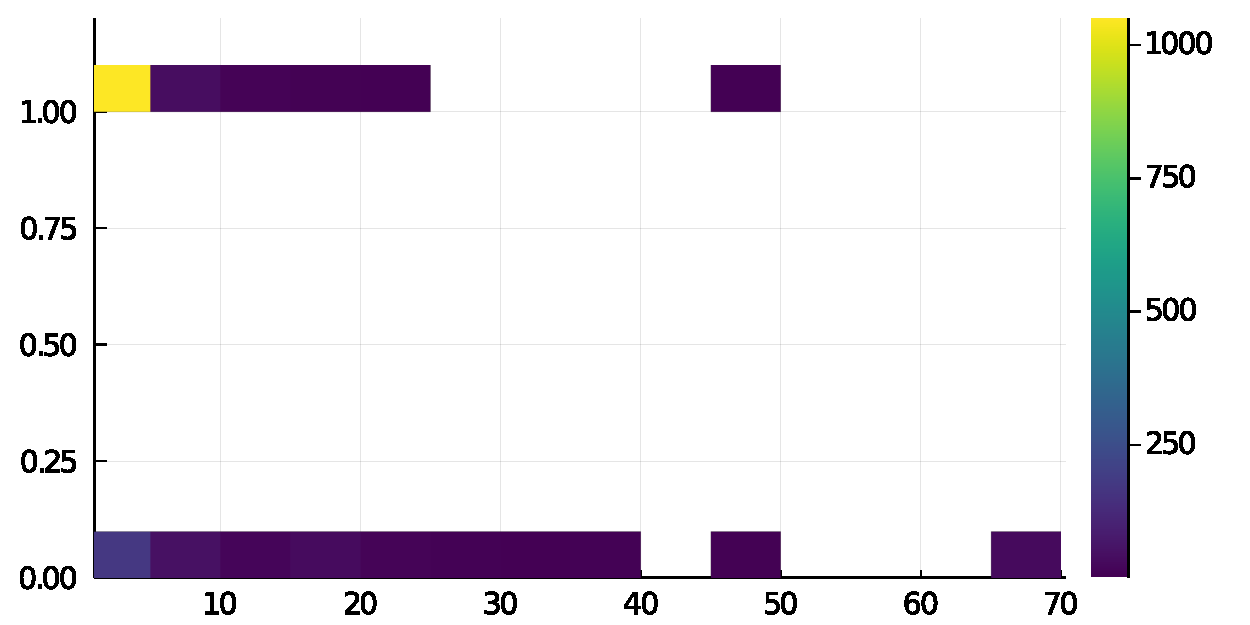
\includegraphics[width=\textwidth]{figs/all-package-graphs/Genie-gotos-vs-grounded.pdf}
     \end{subfigure}
\caption{Stability (left, OY axis) and groundedness (right, OY) by number of gotos in method instances (OX)}%
\Description{Stability and groundedness by number of goto's in method instances in Genie}%
\label{figs:gotos:Genie}
\end{figure}

\begin{figure}[h]
     \begin{subfigure}[b]{0.49\textwidth}
       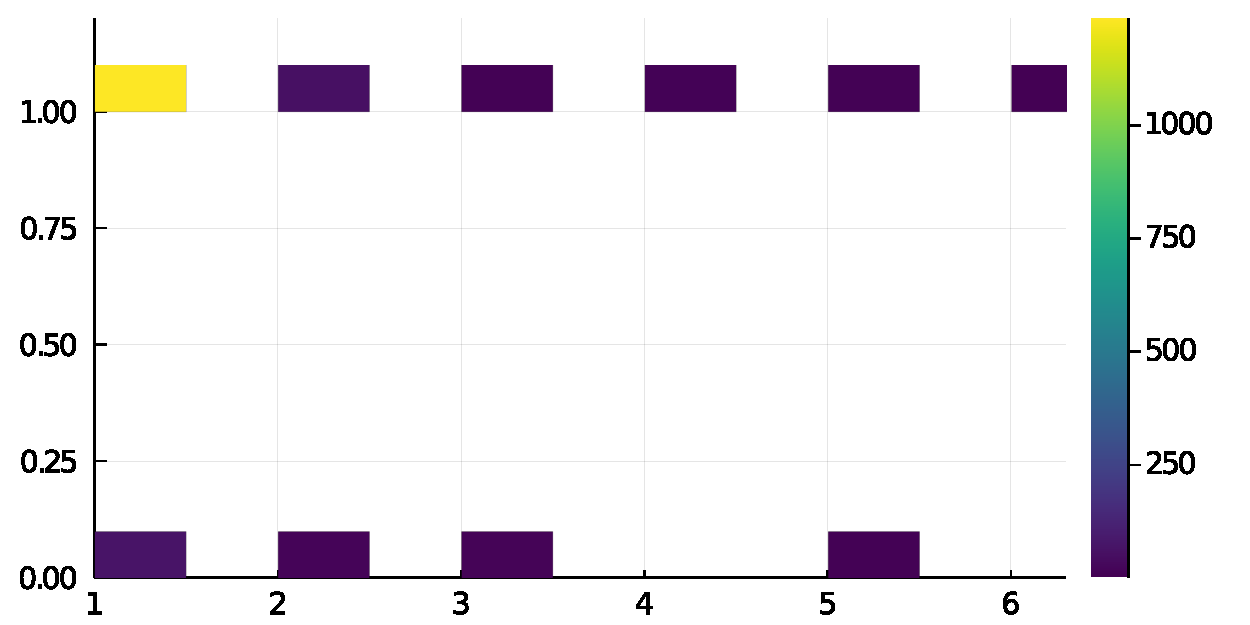
\includegraphics[width=\textwidth]{figs/all-package-graphs/Genie-returns-vs-stable.pdf}
     \end{subfigure}
     \ \
     \begin{subfigure}[b]{0.49\textwidth}
       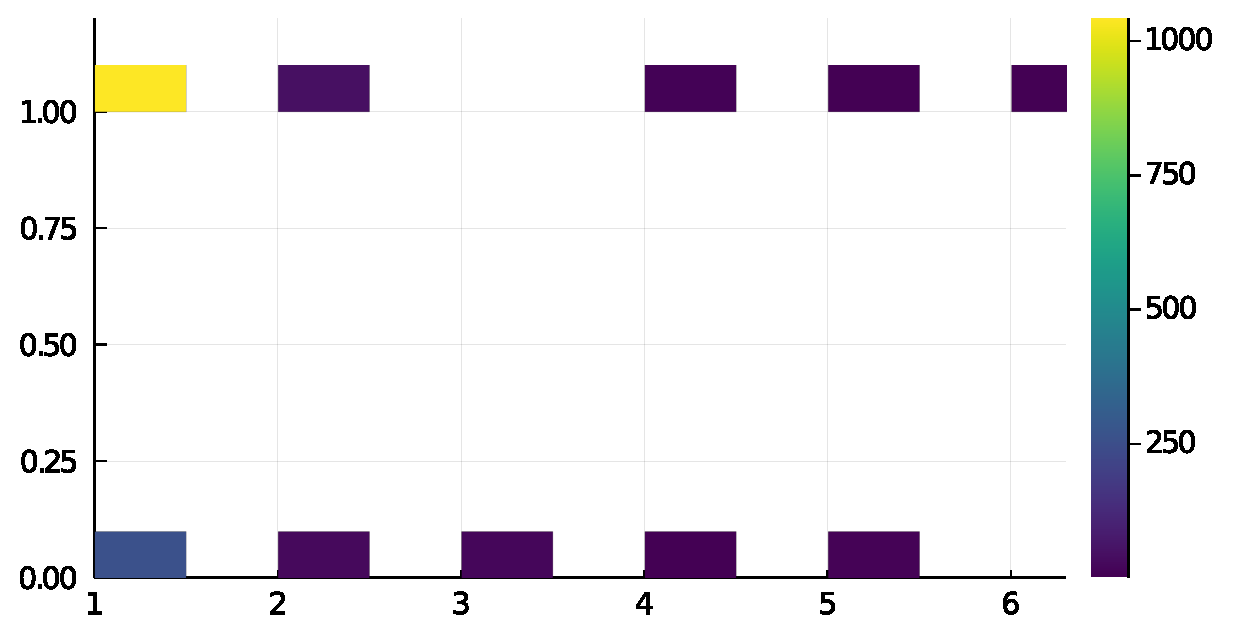
\includegraphics[width=\textwidth]{figs/all-package-graphs/Genie-returns-vs-grounded.pdf}
     \end{subfigure}
\caption{Stability (left, OY axis) and groundedness (right, OY) by number of returns in method instances (OX)}%
\Description{Stability and groundedness by number of returns in method instances in Genie}%
\label{figs:returns:Genie}
\end{figure}
\clearpage
\subsection{Package: IJulia}
\begin{figure}[h]
     \begin{subfigure}[b]{0.49\textwidth}
       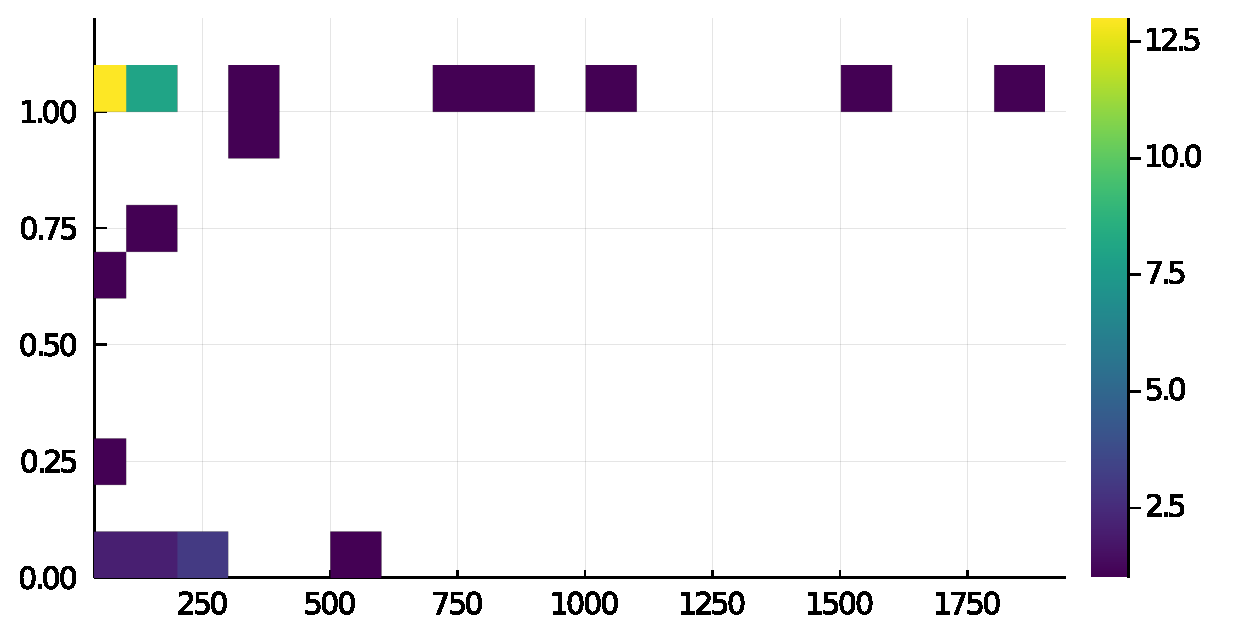
\includegraphics[width=\textwidth]{figs/all-package-graphs/IJulia-size-vs-stable.pdf}
     \end{subfigure}
     \ \
     \begin{subfigure}[b]{0.49\textwidth}
       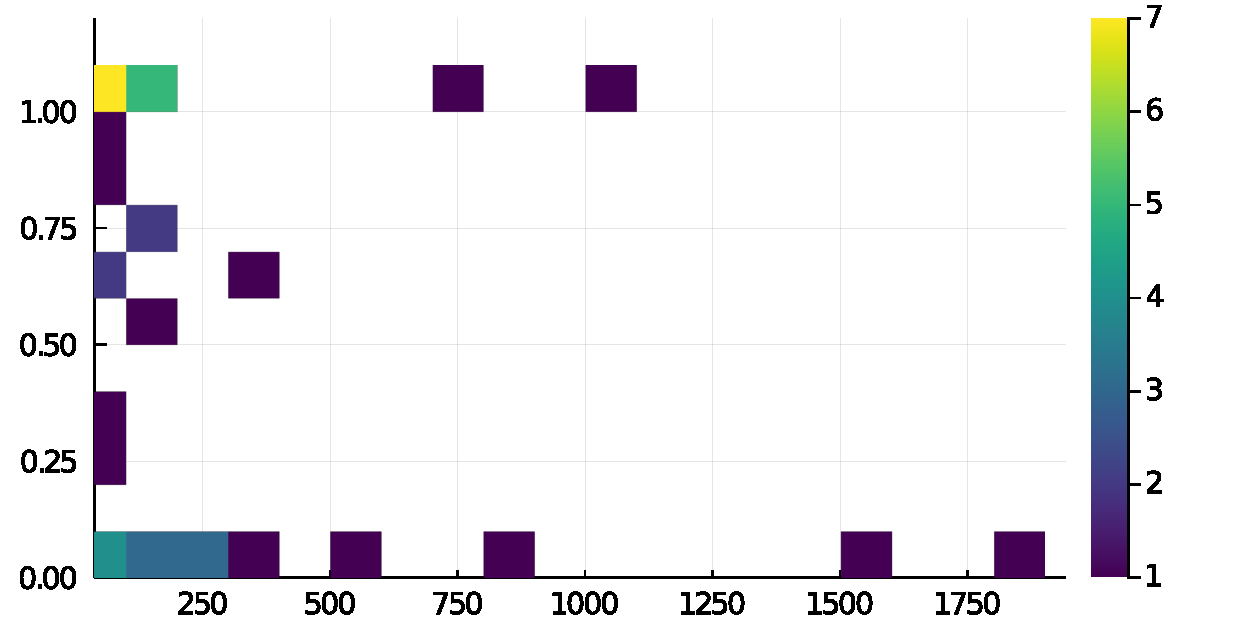
\includegraphics[width=\textwidth]{figs/all-package-graphs/IJulia-size-vs-grounded.pdf}
     \end{subfigure}
\caption{Stability (left, OY axis) and groundedness (right, OY) by method size (OX)}%
\Description{Stability and groundedness by method size in IJulia}%
\label{figs:size:IJulia}
\end{figure}

\begin{figure}[h]
     \begin{subfigure}[b]{0.49\textwidth}
       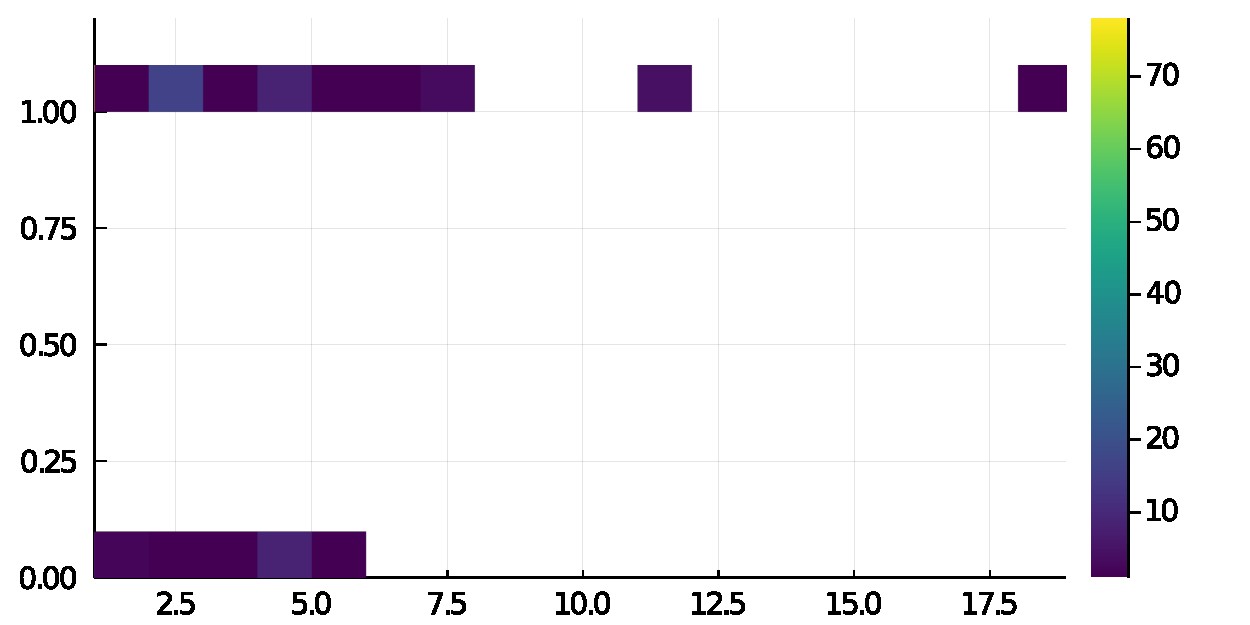
\includegraphics[width=\textwidth]{figs/all-package-graphs/IJulia-gotos-vs-stable.pdf}
     \end{subfigure}
     \ \
     \begin{subfigure}[b]{0.49\textwidth}
       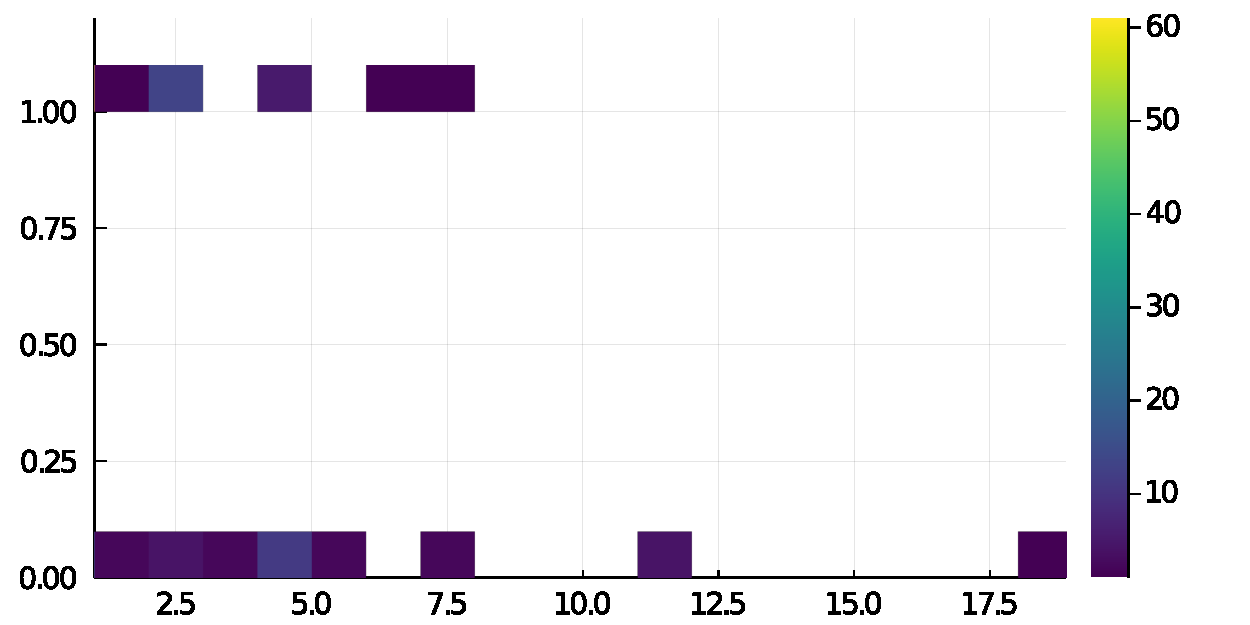
\includegraphics[width=\textwidth]{figs/all-package-graphs/IJulia-gotos-vs-grounded.pdf}
     \end{subfigure}
\caption{Stability (left, OY axis) and groundedness (right, OY) by number of gotos in method instances (OX)}%
\Description{Stability and groundedness by number of goto's in method instances in IJulia}%
\label{figs:gotos:IJulia}
\end{figure}

\begin{figure}[h]
     \begin{subfigure}[b]{0.49\textwidth}
       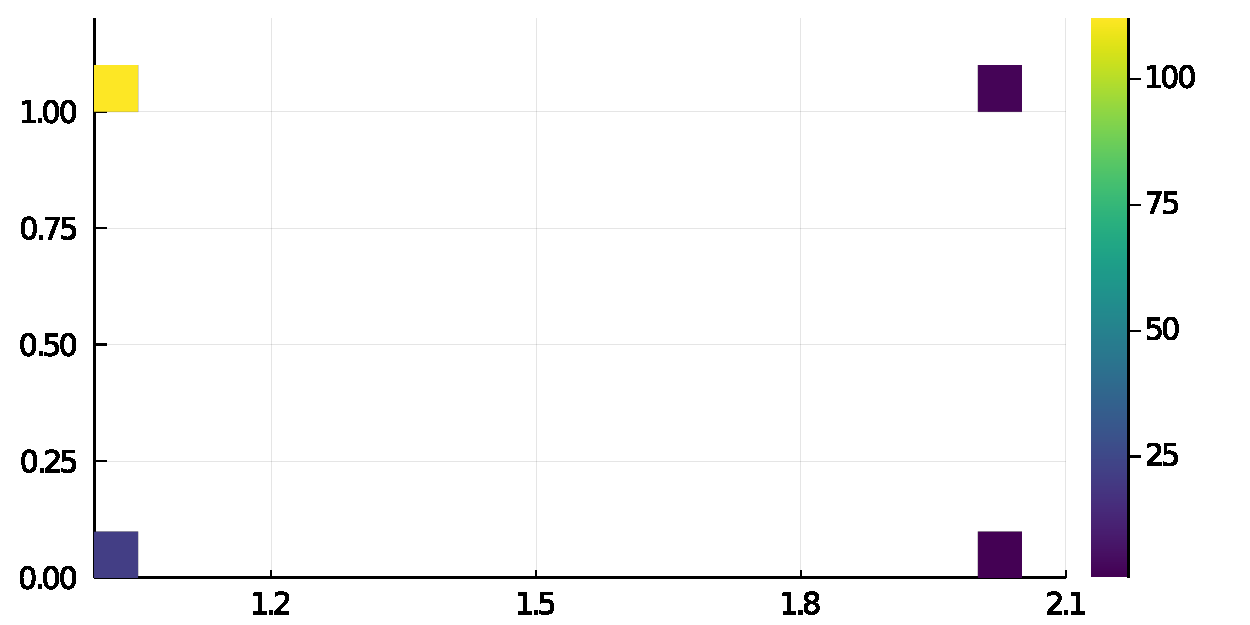
\includegraphics[width=\textwidth]{figs/all-package-graphs/IJulia-returns-vs-stable.pdf}
     \end{subfigure}
     \ \
     \begin{subfigure}[b]{0.49\textwidth}
       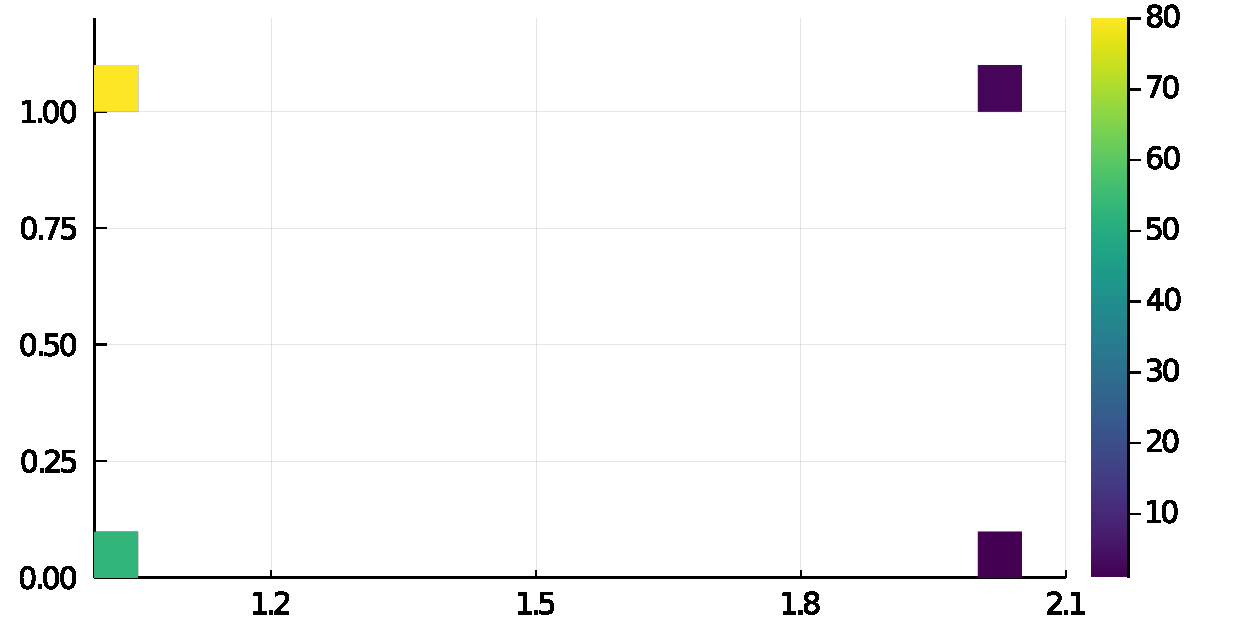
\includegraphics[width=\textwidth]{figs/all-package-graphs/IJulia-returns-vs-grounded.pdf}
     \end{subfigure}
\caption{Stability (left, OY axis) and groundedness (right, OY) by number of returns in method instances (OX)}%
\Description{Stability and groundedness by number of returns in method instances in IJulia}%
\label{figs:returns:IJulia}
\end{figure}
\clearpage
\subsection{Package: JuMP}
\begin{figure}[h]
     \begin{subfigure}[b]{0.49\textwidth}
       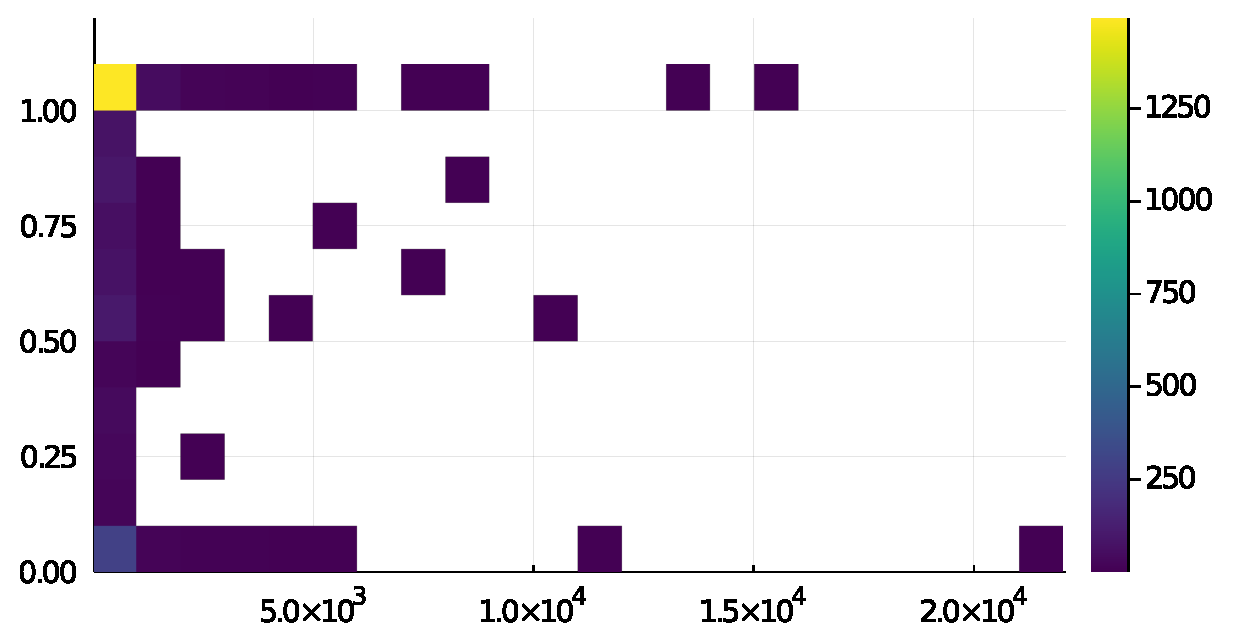
\includegraphics[width=\textwidth]{figs/all-package-graphs/JuMP-size-vs-stable.pdf}
     \end{subfigure}
     \ \
     \begin{subfigure}[b]{0.49\textwidth}
       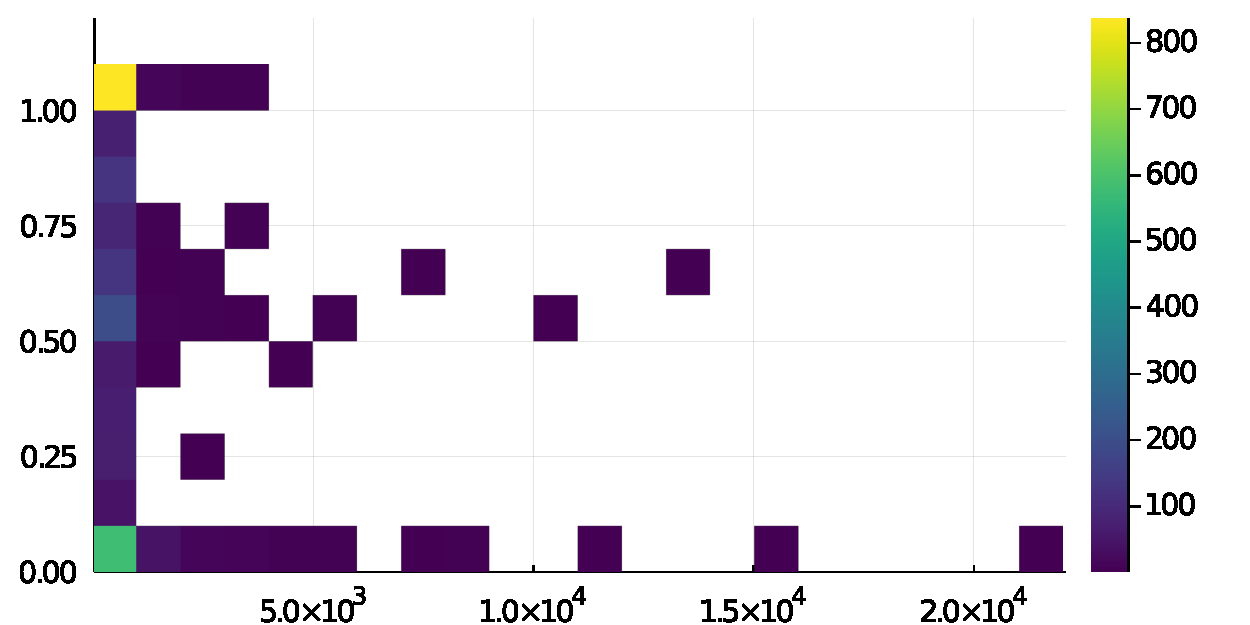
\includegraphics[width=\textwidth]{figs/all-package-graphs/JuMP-size-vs-grounded.pdf}
     \end{subfigure}
\caption{Stability (left, OY axis) and groundedness (right, OY) by method size (OX)}%
\Description{Stability and groundedness by method size in JuMP}%
\label{figs:size:JuMP}
\end{figure}

\begin{figure}[h]
     \begin{subfigure}[b]{0.49\textwidth}
       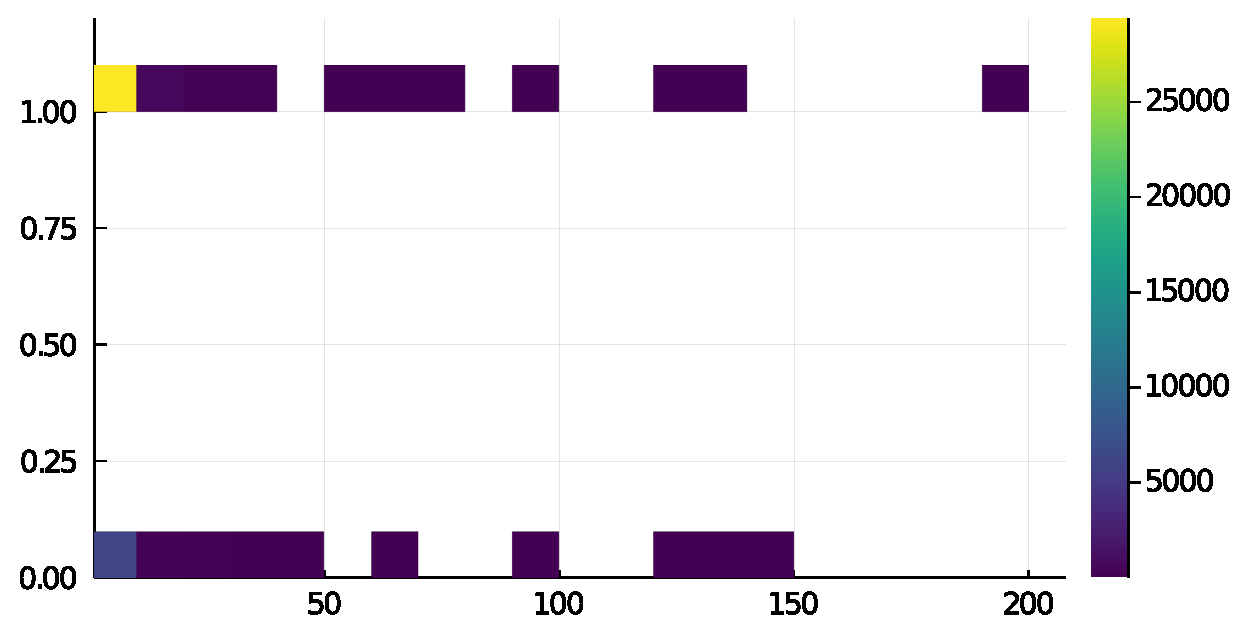
\includegraphics[width=\textwidth]{figs/all-package-graphs/JuMP-gotos-vs-stable.pdf}
     \end{subfigure}
     \ \
     \begin{subfigure}[b]{0.49\textwidth}
       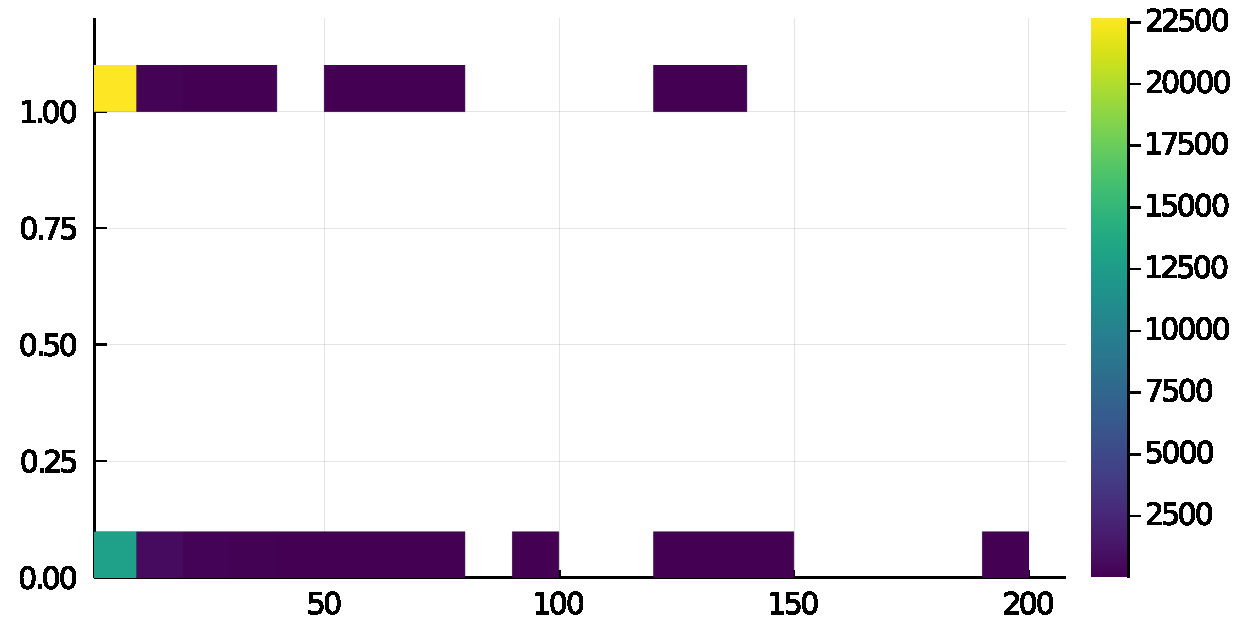
\includegraphics[width=\textwidth]{figs/all-package-graphs/JuMP-gotos-vs-grounded.pdf}
     \end{subfigure}
\caption{Stability (left, OY axis) and groundedness (right, OY) by number of gotos in method instances (OX)}%
\Description{Stability and groundedness by number of goto's in method instances in JuMP}%
\label{figs:gotos:JuMP}
\end{figure}

\begin{figure}[h]
     \begin{subfigure}[b]{0.49\textwidth}
       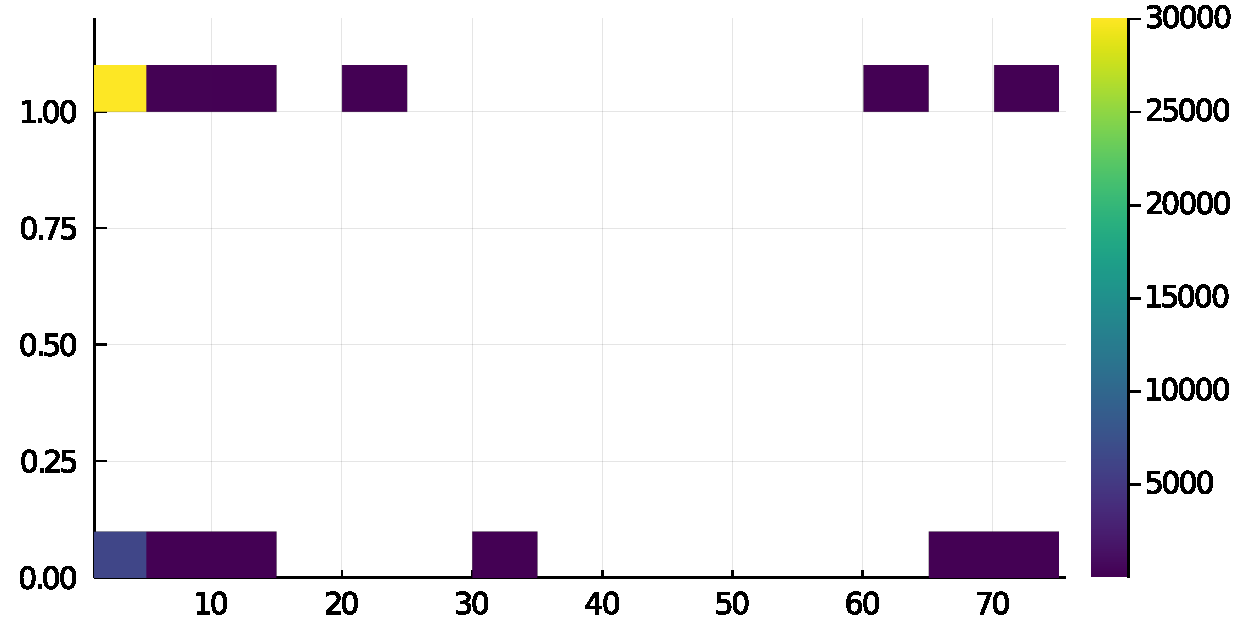
\includegraphics[width=\textwidth]{figs/all-package-graphs/JuMP-returns-vs-stable.pdf}
     \end{subfigure}
     \ \
     \begin{subfigure}[b]{0.49\textwidth}
       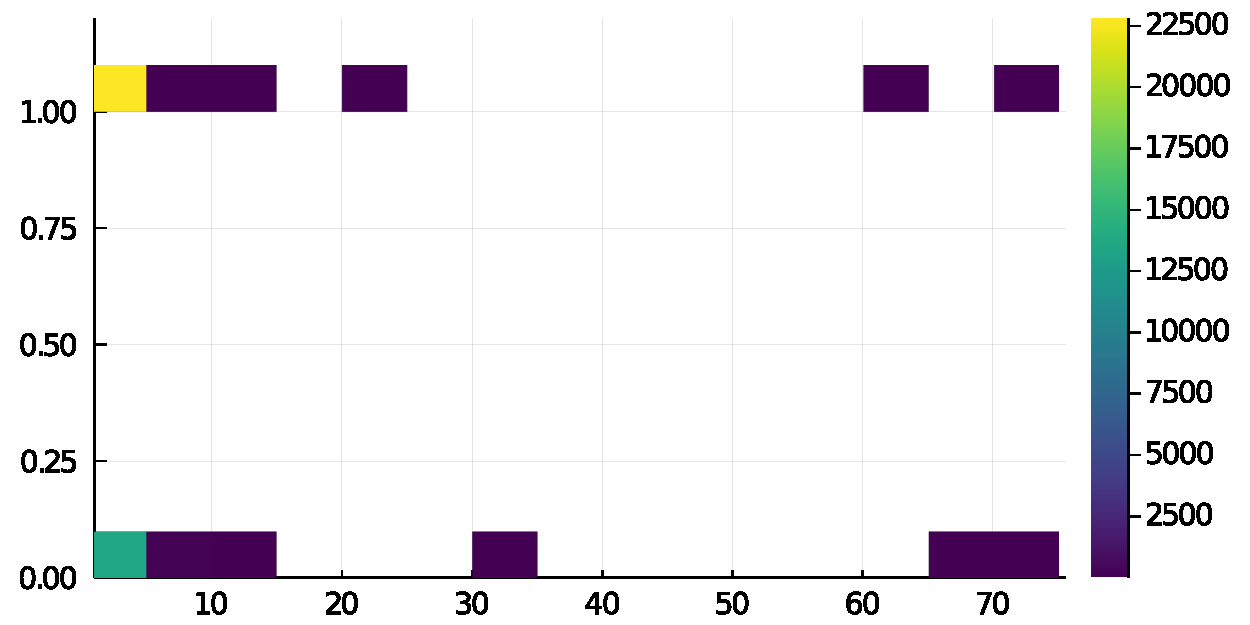
\includegraphics[width=\textwidth]{figs/all-package-graphs/JuMP-returns-vs-grounded.pdf}
     \end{subfigure}
\caption{Stability (left, OY axis) and groundedness (right, OY) by number of returns in method instances (OX)}%
\Description{Stability and groundedness by number of returns in method instances in JuMP}%
\label{figs:returns:JuMP}
\end{figure}
\clearpage
\subsection{Package: Knet}
\begin{figure}[h]
     \begin{subfigure}[b]{0.49\textwidth}
       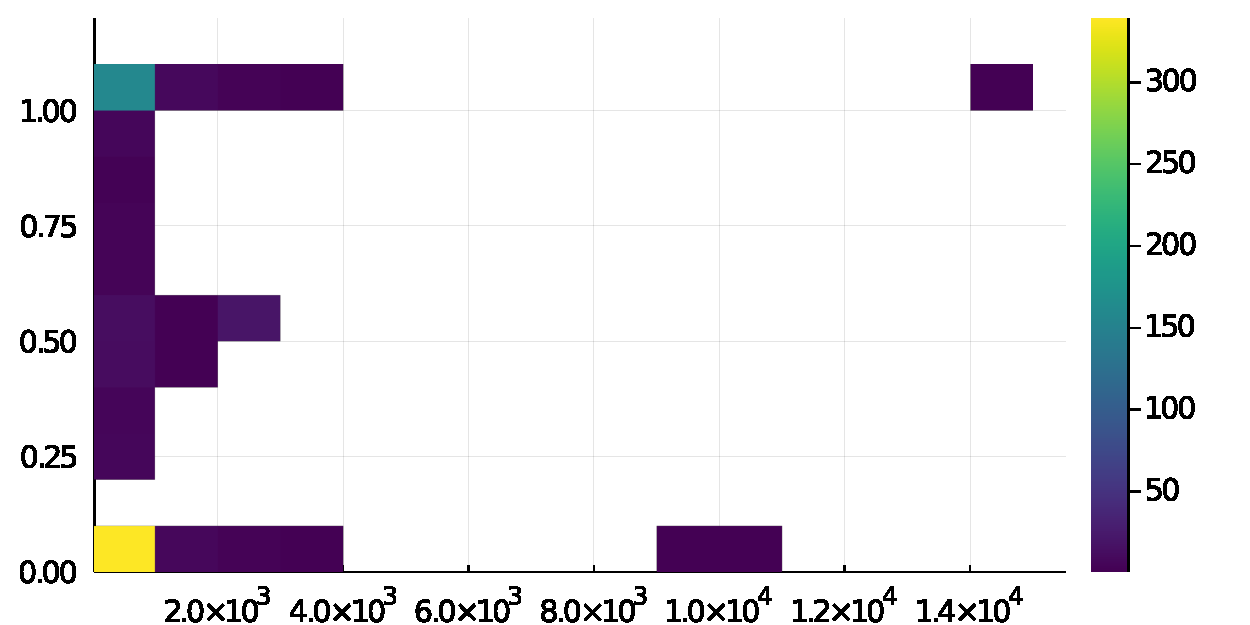
\includegraphics[width=\textwidth]{figs/all-package-graphs/Knet-size-vs-stable.pdf}
     \end{subfigure}
     \ \
     \begin{subfigure}[b]{0.49\textwidth}
       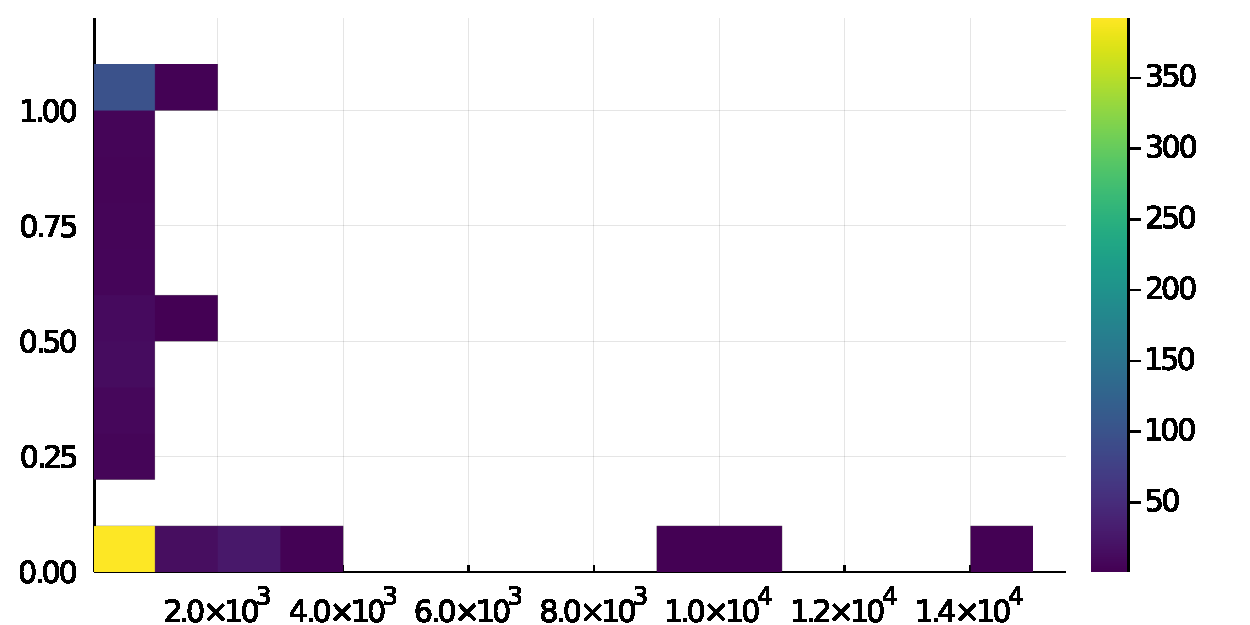
\includegraphics[width=\textwidth]{figs/all-package-graphs/Knet-size-vs-grounded.pdf}
     \end{subfigure}
\caption{Stability (left, OY axis) and groundedness (right, OY) by method size (OX)}%
\Description{Stability and groundedness by method size in Knet}%
\label{figs:size:Knet}
\end{figure}

\begin{figure}[h]
     \begin{subfigure}[b]{0.49\textwidth}
       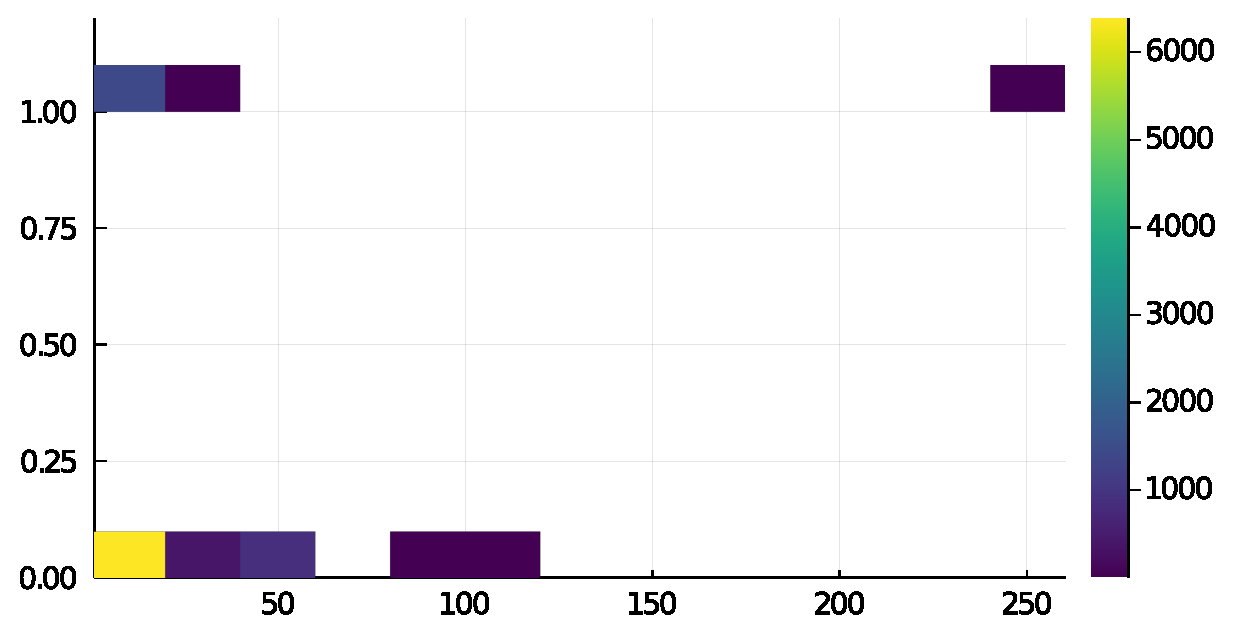
\includegraphics[width=\textwidth]{figs/all-package-graphs/Knet-gotos-vs-stable.pdf}
     \end{subfigure}
     \ \
     \begin{subfigure}[b]{0.49\textwidth}
       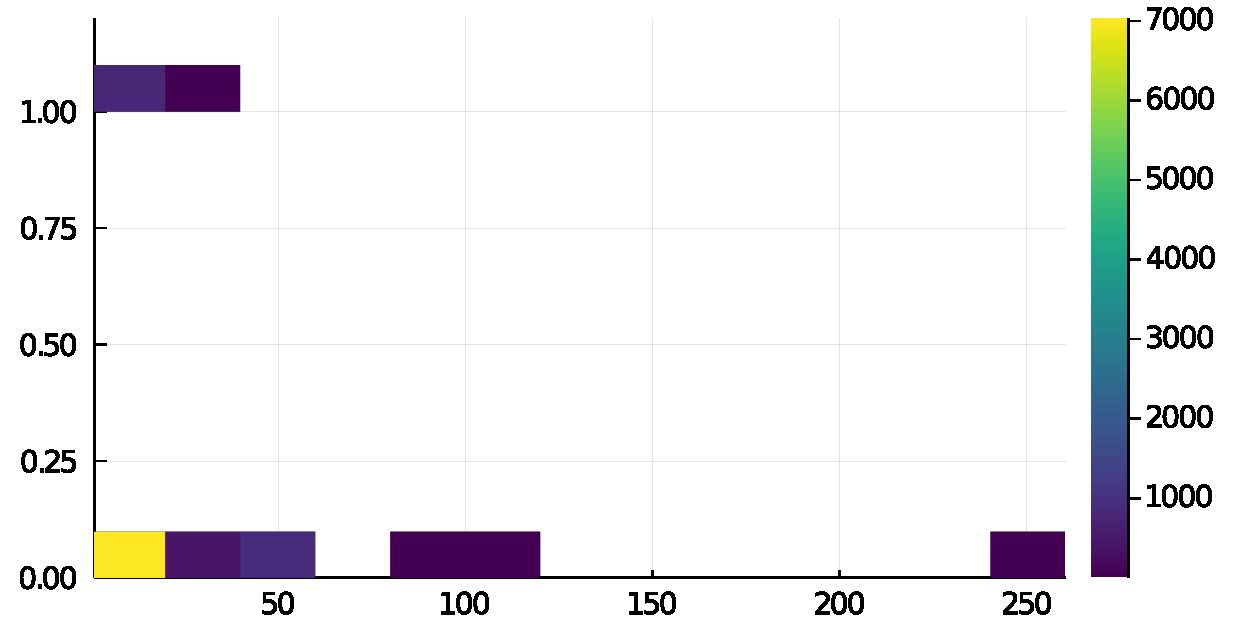
\includegraphics[width=\textwidth]{figs/all-package-graphs/Knet-gotos-vs-grounded.pdf}
     \end{subfigure}
\caption{Stability (left, OY axis) and groundedness (right, OY) by number of gotos in method instances (OX)}%
\Description{Stability and groundedness by number of goto's in method instances in Knet}%
\label{figs:gotos:Knet}
\end{figure}

\begin{figure}[h]
     \begin{subfigure}[b]{0.49\textwidth}
       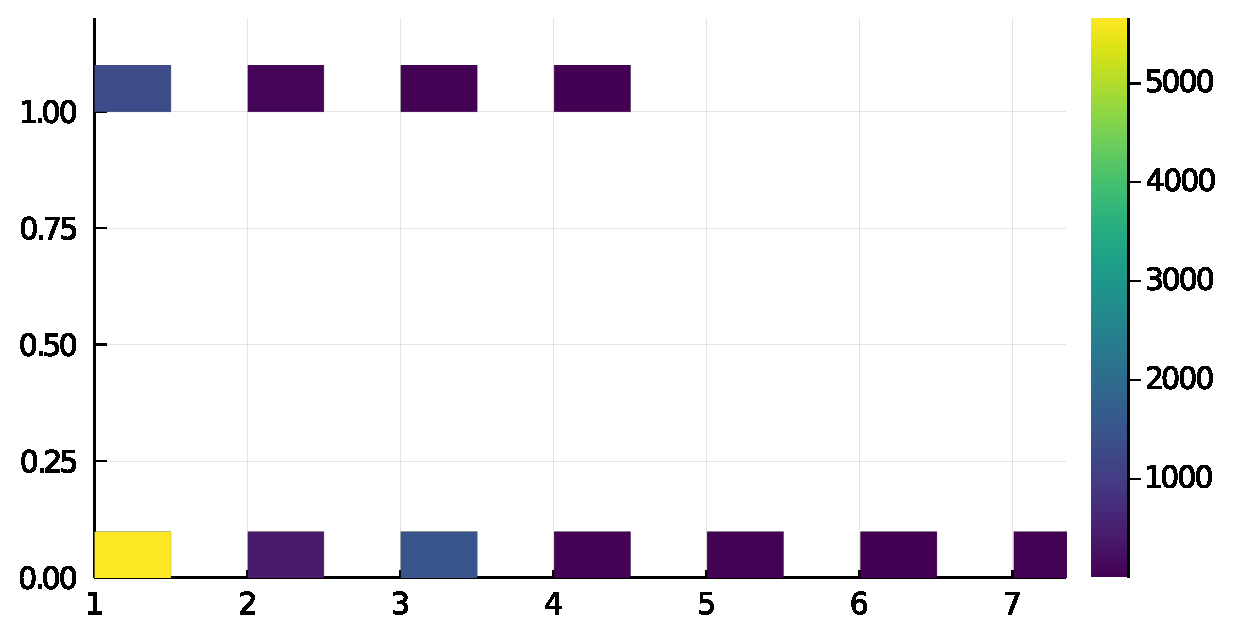
\includegraphics[width=\textwidth]{figs/all-package-graphs/Knet-returns-vs-stable.pdf}
     \end{subfigure}
     \ \
     \begin{subfigure}[b]{0.49\textwidth}
       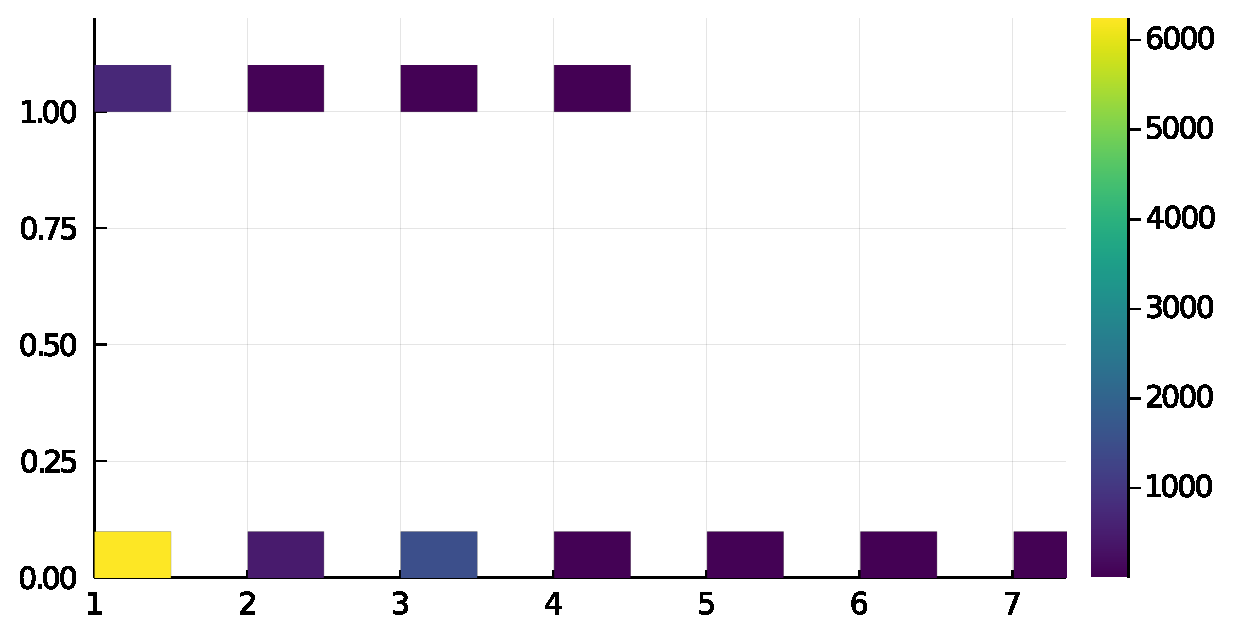
\includegraphics[width=\textwidth]{figs/all-package-graphs/Knet-returns-vs-grounded.pdf}
     \end{subfigure}
\caption{Stability (left, OY axis) and groundedness (right, OY) by number of returns in method instances (OX)}%
\Description{Stability and groundedness by number of returns in method instances in Knet}%
\label{figs:returns:Knet}
\end{figure}
\clearpage
\subsection{Package: Plots}
\begin{figure}[h]
     \begin{subfigure}[b]{0.49\textwidth}
       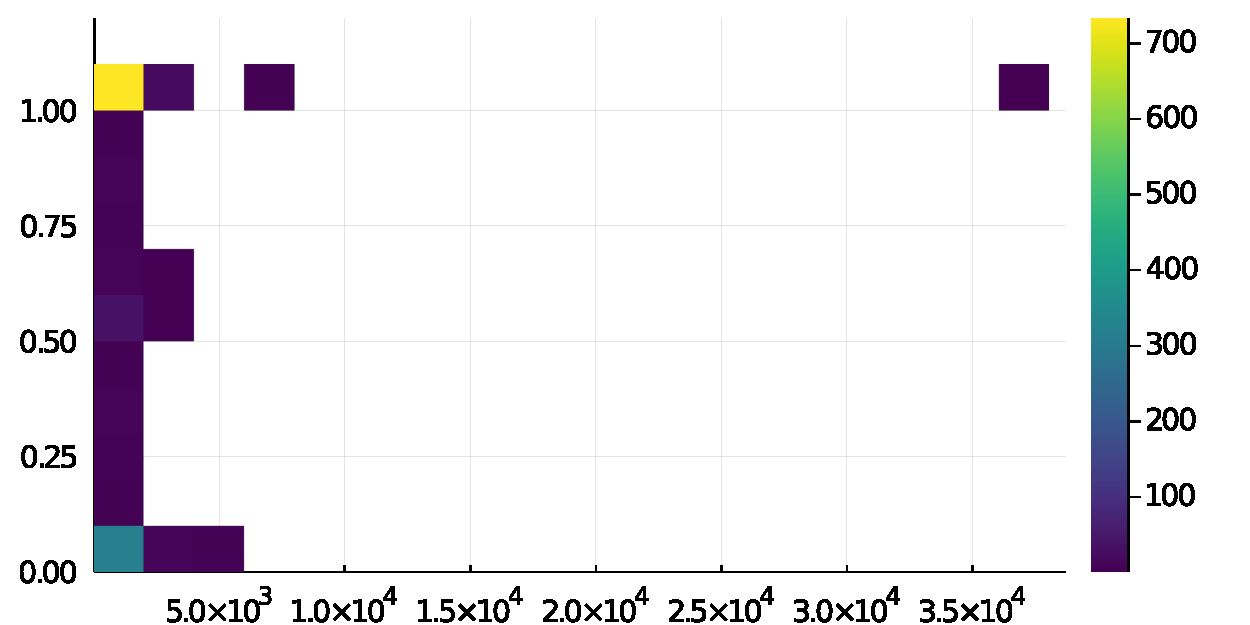
\includegraphics[width=\textwidth]{figs/all-package-graphs/Plots-size-vs-stable.pdf}
     \end{subfigure}
     \ \
     \begin{subfigure}[b]{0.49\textwidth}
       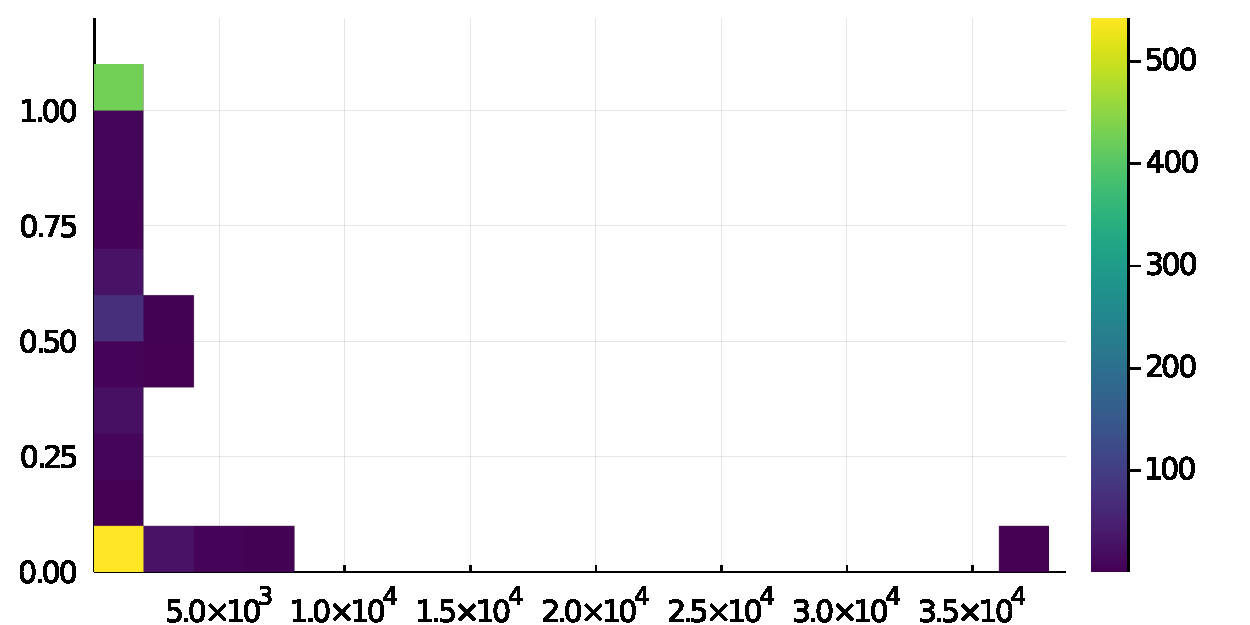
\includegraphics[width=\textwidth]{figs/all-package-graphs/Plots-size-vs-grounded.pdf}
     \end{subfigure}
\caption{Stability (left, OY axis) and groundedness (right, OY) by method size (OX)}%
\Description{Stability and groundedness by method size in Plots}%
\label{figs:size:Plots}
\end{figure}

\begin{figure}[h]
     \begin{subfigure}[b]{0.49\textwidth}
       \includegraphics[width=\textwidth]{figs/all-package-graphs/Plots-gotos-vs-stable.pdf}
     \end{subfigure}
     \ \
     \begin{subfigure}[b]{0.49\textwidth}
       \includegraphics[width=\textwidth]{figs/all-package-graphs/Plots-gotos-vs-grounded.pdf}
     \end{subfigure}
\caption{Stability (left, OY axis) and groundedness (right, OY) by number of gotos in method instances (OX)}%
\Description{Stability and groundedness by number of goto's in method instances in Plots}%
\label{figs:gotos:Plots}
\end{figure}

\begin{figure}[h]
     \begin{subfigure}[b]{0.49\textwidth}
       \includegraphics[width=\textwidth]{figs/all-package-graphs/Plots-returns-vs-stable.pdf}
     \end{subfigure}
     \ \
     \begin{subfigure}[b]{0.49\textwidth}
       \includegraphics[width=\textwidth]{figs/all-package-graphs/Plots-returns-vs-grounded.pdf}
     \end{subfigure}
\caption{Stability (left, OY axis) and groundedness (right, OY) by number of returns in method instances (OX)}%
\Description{Stability and groundedness by number of returns in method instances in Plots}%
\label{figs:returns:Plots}
\end{figure}
\clearpage
\subsection{Package: Pluto}
\begin{figure}[h]
     \begin{subfigure}[b]{0.49\textwidth}
       \includegraphics[width=\textwidth]{figs/all-package-graphs/Pluto-size-vs-stable.pdf}
     \end{subfigure}
     \ \
     \begin{subfigure}[b]{0.49\textwidth}
       \includegraphics[width=\textwidth]{figs/all-package-graphs/Pluto-size-vs-grounded.pdf}
     \end{subfigure}
\caption{Stability (left, OY axis) and groundedness (right, OY) by method size (OX)}%
\Description{Stability and groundedness by method size in Pluto}%
\label{figs:size:Pluto}
\end{figure}

\begin{figure}[h]
     \begin{subfigure}[b]{0.49\textwidth}
       \includegraphics[width=\textwidth]{figs/all-package-graphs/Pluto-gotos-vs-stable.pdf}
     \end{subfigure}
     \ \
     \begin{subfigure}[b]{0.49\textwidth}
       \includegraphics[width=\textwidth]{figs/all-package-graphs/Pluto-gotos-vs-grounded.pdf}
     \end{subfigure}
\caption{Stability (left, OY axis) and groundedness (right, OY) by number of gotos in method instances (OX)}%
\Description{Stability and groundedness by number of goto's in method instances in Pluto}%
\label{figs:gotos:Pluto}
\end{figure}

\begin{figure}[h]
     \begin{subfigure}[b]{0.49\textwidth}
       \includegraphics[width=\textwidth]{figs/all-package-graphs/Pluto-returns-vs-stable.pdf}
     \end{subfigure}
     \ \
     \begin{subfigure}[b]{0.49\textwidth}
       \includegraphics[width=\textwidth]{figs/all-package-graphs/Pluto-returns-vs-grounded.pdf}
     \end{subfigure}
\caption{Stability (left, OY axis) and groundedness (right, OY) by number of returns in method instances (OX)}%
\Description{Stability and groundedness by number of returns in method instances in Pluto}%
\label{figs:returns:Pluto}
\end{figure}
\clearpage

